\documentclass{thesisby}

%\usepackage[cp1251]{inputenc}
\usepackage[utf8]{inputenc}
\usepackage[T2A]{fontenc}
\usepackage[russian]{babel}

%\usepackage{pscyr}
%\renewcommand{\rmdefault}{ftm}

%для борьбы с переполнениями за счет разреженных слов в абзаце
\emergencystretch=25pt
%math
\usepackage{mathtools}
\usepackage{tabularx}
\usepackage{pdflscape}

\usepackage{afterpage}
\usepackage{geometry}
\usepackage{multirow}
\usepackage{enumitem}

\usepackage{amsmath,amssymb,amsfonts}
\usepackage{longtable,array}
\usepackage{graphicx,epsfig}
\usepackage[unicode,colorlinks=false,pagebackref=false, hidelinks]{hyperref}
\urlstyle{same}
%\usepackage{refcheck}% checks lost and useless labels, shows `keys' of \label in the margins
%фиксить картинки
%\usepackage{float}

\usepackage{textcomp}% For Celsium sign only

% Листинги с исходным кодом программ
\usepackage{fancyvrb}
\usepackage{listings}
\usepackage{totcount}
%\usepackage{totpages}
\usepackage{cite}

% Плавающие окружения. во многом лучше пакета float
\usepackage{floatrow}

\usepackage{tikz}
\newcolumntype{P}[1]{>{\centering\arraybackslash}p{#1}}
\newcolumntype{M}[1]{>{\centering\arraybackslash}m{#1}}

%for lists
\usepackage[ampersand]{easylist}
\ListProperties(Hide=100, Hang=false, Margin=0mm, Indent1=10.5mm, Indent2=15mm, Style*=-- ,
Style2*=$\bullet$ ,Style3*=$\circ$ ,Style4*=\tiny$\blacksquare$ )

\usepackage[ruled, vlined]{algorithm2e}
\makeatletter
\newenvironment{algo}[1][]
  {\renewcommand{\algorithmcfname}{Алгоритм}%
   \begin{algorithm}[#1]
   \long\def\@caption##1[##2]##3{%
     \par
     \begingroup\@parboxrestore
     \if@minipage\@setminipage\fi
     \normalsize \@makecaption{\AlCapSty{\AlCapFnt\algorithmcfname}}{\ignorespaces ##3}%
     \par\endgroup
   }}
  {\end{algorithm}}
\makeatother

% \SetKwData{KwDat}{Данные}
\SetKwInput{KwIn}{Исходные данные}
\SetKwInput{KwRes}{Результат}%
% \SetKwIF{Si}{SinonSi}{Sinon}{si}{alors}{sinon si}{sinon}{fin si}%
% \SetKwFor{Tq}{tant que}{faire}{fin tq}%

\newenvironment{easylistNum}{\begin{easylist}
\ListProperties(Hide1=0, Hang=false, Margin=0mm, Indent1=10.5mm, Indent2=15mm, Start1=1, Style*=, FinalMark={)})}{\ListProperties(Hide=100, Hang=false, Margin=0mm, Indent1=10.5mm, Indent2=15mm, Style*=-- ,
Style2*=$\bullet$ ,Style3*=$\circ$ ,Style4*=\tiny$\blacksquare$ )\end{easylist}}

\renewcommand\labelitemi{\textbf{--}}
\floatsetup[table]{capposition=top}

    % \lstset{
    %     language=Python,
    %     basicstyle=\ttfamily,
    %     keywordstyle=\bfseries,
    %     showspaces=false,
    %     showstringspaces=false,
    %     mathescape=true,
    %     aboveskip=0pt,
    %     belowskip=6pt
    % }
\lstdefinestyle{PythonStyle}{
  keywordstyle=\bf,
  belowcaptionskip=1\baselineskip,
  breaklines=true,
  language=Python,
  showstringspaces=false,
  basicstyle=\small\ttfamily,
  commentstyle=\itshape
}
% \lstdefinestyle{PythonStyle}{
% basicstyle=\footnotesize\ttfamily,
% language=Python,
% keywordstyle=\bfseries,
% showstringspaces=false,
% commentstyle={},
% texcl=true
% }

\graphicspath{{../}}

%\renewcommand{\cftchapleader}{\cftdotfill{\cftdotsep}}


\def\isabstract{1}

\begin{document}

\thispagestyle{empty}

\begin{center} 

\bfseries
%{Учреждение образования}
\medskip

{БЕЛОРУССКИЙ ГОСУДАРСТВЕННЫЙ УНИВЕРСИТЕТ}
%{БЕЛОРУССКИЙ ГОСУДАРСТВЕННЫЙ УНИВЕРСИТЕТ ИНФОРМАТИКИ И РАДИОЭЛЕКТРОНИКИ}

%\vspace*{\fill}

\vspace{2cm}
\end{center}

\noindent Объект авторского права\\
\noindent УДК 004.032.26 \\[5mm]

\begin{center}

{КРОЩЕНКО \\ Александр Александрович}\\

%\vspace*{\fill}
\vspace{1cm}

{\bfseries МЕТОДЫ ОБУЧЕНИЯ ГЛУБОКИХ НЕЙРОННЫХ СЕТЕЙ 
ДЛЯ ЗАДАЧ КОМПЬЮТЕРНОГО ЗРЕНИЯ}\\ \vspace{2cm}

АВТОРЕФЕРАТ\\ диссертации на соискание ученой степени\\
кандидата технических наук\\
\medskip


%\vspace*{\fill}

    
\vspace{1cm}
по специальности 05.13.17 -- Теоретические основы информатики 

\vspace*{\fill}


Минск 2024
\end{center}


\newpage

\thispagestyle{empty} 

\noindent Научная работа выполнена\\ в \textbf{УО <<Брестский государственный технический университет>>}.

\vspace*{\fill} 

 

\noindent \hangindent=53mm
     Научный руководитель -- \\ {\bf Головко Владимир Адамович}, доктор технических наук, профессор, заведующий кафедрой интеллектуальных информационных технологий УО <<Брестский государственный технический университет>>.\\
            
\vspace*{\fill} \noindent \hangindent=53mm
    Официальные оппоненты:\\ {\bf Старовойтов Валерий Васильевич},\\ доктор технических наук, профессор,; %профессор кафедры электронных вычислительных машин учреждения образования <<Белорусский государственный университет информатики и радиоэлектроники>>
    \\ [5pt]
    {\bf Лукашевич Марина Михайловна},\\ кандидат технических наук, доцент, доцент кафедры информационных систем управления факультета прикладной математики и информатики БГУ.

\vspace*{\fill} \noindent \hangindent=53mm Оппонирующая
организация -- \\\textbf{Белорусский государственный университет информатики и радиоэлектроники.}

\vspace*{\fill} \noindent Защита состоится \textbf{число февраля~2024~года} в \textit{10.00} часов на заседании совета по защите диссертаций Д 02.01.02 при Белорусском государственном университете (\textit{г. Минск, ул. Ленинградская 8, корпус юридического факультета}), \textit{ауд. 407}. Телефон ученого секретаря 209-57-09.\\
Почтовый адрес: пр-т Независимости 4, Минск, 220030.\\
Телефон ученого секретаря: 209-57-09; е-mail: Kochyn@bsu.by.

\vspace*{\fill} \noindent
С диссертацией можно ознакомиться в Фундаментальной библиотеке\\ Белорусского государственного университета.

\vspace*{\fill} \noindent
Автореферат разослан~\textit{<<\rule{10mm}{0.4pt}>>~января~2024~года}.
%~\rule{25mm}{0.4pt}~1999~г.

\vspace*{\fill}

\noindent Ученый секретарь совета \\ по защите диссертаций \\ кандидат технических наук доцент
\hfill В.П.~Кочин

\vspace*{\fill}

\vspace*{\fill}

\newpage
\setcounter{page}{1}

\centerline{\bf ВВЕДЕНИЕ}

\parindent=1cm

\medskip
% В настоящее время все более актуальным становится использование интеллектуальных систем в самых различных областях. Одним из ключевых компонентов интеллектуальной системы, обеспечивающим возможность решать широкий круг задач, является решатель задач. Особенностью решателей задач интеллектуальных систем по сравнению с другими современными программными системами является необходимость решать задачи в условиях, когда сведения, необходимые для решения задачи, не локализованы явно в базе знаний интеллектуальной системы и должны быть найдены в процессе решения задачи на основании каких-либо критериев.

% \ifx\isabstract\undefined 
% Состав решателя задач каждой конкретной системы зависит от ее назначения, классов решаемых задач, предметной области и ряда других факторов.
% \fi

% \ifx\isabstract\undefined 
% В общем случае решатель задач обеспечивает возможность решения задач, связанных как с непосредственно основной функциональностью системы, так и с обеспечением эффективности работы такой системы, а также с обеспечением автоматизации развития самой этой системы. Решатель задач, обеспечивающий выполнение всех перечисленных функций, будем называть \textit{объединенным решателем задач} указанной интеллектуальной системы.
% \fi

% %Ключевой отличительной особенностью решателей задач от современных программных систем вообще является необходимость решать задачи в условиях, когда исходные данные для задачи не локализованы явно
% %Отличительными особенностями решателей задач является их ориентация на обработку знаний, хранящихся в базе знаний интеллектуальной системы, а также 

% Расширение областей применения интеллектуальных систем требует от таких систем возможности решения комплексных задач, решение каждой из которых предполагает совместное использование целого ряда различных моделей представления знаний и различных моделей решения задач. Кроме того, решение комплексных задач предполагает использование общих информационных ресурсов (в предельном случае -- всей базы знаний интеллектуальной системы) различными компонентами решателя, ориентированными на решение различных подзадач. Поскольку решатель комплексных задач осуществляет интеграцию различных моделей решения задач, будем называть его \textit{гибридным решателем задач}.

% Примерами комплексных задач являются:

% \begin{easylist}
% &	задачи понимания текстов естественного языка (как печатных, так и рукописных), понимания речевых сообщений, изображений\ifx\isabstract\undefined. В каждом из перечисленных случаев необходимо осуществить синтаксический анализ обрабатываемого файла (сигнала), устранить незначимые фрагменты, классифицировать значимые фрагменты, соотнести их с понятиями, известными системе, выявить те фрагменты, которые система распознать не в состоянии, устранить дублирование информации и т. д.\fi;
% &	задачи автоматизации адаптивного обучения школьников и студентов\ifx\isabstract\undefined, предполагающие, что система может самостоятельно решать различные задачи из некоторой предметной области, а также управлять процессом обучения, самостоятельно формировать задания для учащихся и контролировать их выполнение\fi;
% &	задачи планирования поведения интеллектуальных роботов\ifx\isabstract\undefined, предполагающие как понимание различного рода внешней информации, так и принятие различных решений с использованием как достоверных методов, так и правдоподобных\fi;
% &	задачи комплексной и гибкой автоматизации различных предприятий;
% &	и другие.
% \end{easylist}

% Использование различных моделей решения задач в рамках
% интеллектуальной системы предполагает декомпозицию комплексной задачи на подзадачи, которые могут быть решены с помощью одной из известных интеллектуальной системе моделей решения задач. Благодаря комбинации различных моделей решения задач, множество задач, решаемых гибридным решателем, будет значительно шире, чем объединение множеств задач, решаемых по отдельности всеми решателями задач, входящими в его состав\ifx\isabstract\undefined ~\cite{Tarasov2007}\fi.

% \ifx\isabstract\undefined
% Значительный вклад в разработку и исследование моделей, методов и средств решения задач в интеллектуальных системах внесли такие ученые, как E. W. Dijkstra, C. A. Hoare, P. Jackson, J. McCarthy, A. Newell, P. Norvig, G. Polya, R. Reiter, S. Russel, H. A. Simon, D. Waterman, M. Wooldridge, А. Н. Аверкин, И. З. Батыршин, А. Н. Борисов, В. Б. Борщев, В. Н. Вагин, Т. А. Гаврилова, Л. А. Гладков, В. А. Головко, А. Н. Горбань, В. И. Городецкий, В. В. Грибова, А. П. Еремеев, Ю. А. Загорулько, А. С. Клещев, А. В. Колесников, В. Е. Котов, О. П. Кузнецов, В. М. Курейчик, Д. В. Ландэ, Л. В. Массель, А. С. Нариньяни, Г. С. Осипов, Г. С. Плесневич, Э. В. Попов, Д. А. Поспелов, Г. В. Рыбина, П. О. Скобелев, В. Б. Тарасов, Э. Х. Тыугу, В. К. Финн, И. Б. Фоминых, В. Ф. Хорошевский, А. Е. Янковская и др.
% \fi

% Постоянная эволюция интеллектуальных систем и технологий их разработки делает актуальной не только проблему снижения сроков разработки гибридных решателей задач, но и проблему снижения трудоемкости внесения изменений в состав уже разработанных решателей без необходимости изменения архитектуры всей системы в целом. 

% Современные подходы к построению гибридных решателей задач, как правило, предполагают совмещение разнородных моделей решения задач без какой-либо единой основы, например, посредством специализированных программных интерфейсов между разными компонентами системы, что приводит к существенным накладным расходам при разработке такой системы и в особенности при ее модификации, в том числе при добавлении в систему новой модели решения задач. 

% Таким образом, несмотря на успехи в области разработки решателей задач интеллектуальных систем, остаются нерешенными проблемы, связанные с обеспечением:
% \begin{easylist}
% & совместимости различных частных решателей задач, т. е. возможности их согласованного использования при решении одной и той же комплексной задачи;
% & возможности без существенных накладных расходов модифицировать гибридный решатель непосредственно в процессе эксплуатации интеллектуальной системы, в том числе расширять число используемых моделей решения задач без каких-либо ограничений на вид этих моделей. Такое требование обусловлено тем, что при решении комплексной задачи априори может оказаться неизвестным, какие именно модели решения задач и виды знаний могут потребоваться.
% \end{easylist}

% Важным способом снижения трудоемкости процесса изменения функциональности интеллектуальных систем является накопление библиотек совместимых компонентов решателей, которые позволят значительно снизить как сроки разработки и модификации решателей, так и уровень профессиональных требований к их разработчикам.

% Кроме того, актуальной является проблема создания самих средств разработки гибридных решателей задач, обеспечивающих информационную поддержку и автоматизацию деятельности разработчиков.

Практические приложения компьютерного зрения с каждым годом становятся все более разнообразными. В современном мире компьютерное зрение используется повсеместно -- в сложных производственных и медицинских системах, в интеллектуальных системах интернета вещей и развлекательных приложениях для мобильных устройств.

В качестве основы при разработке таких систем все чаще находят применение глубокие нейросетевые модели. Данные модели показывают впечатляющие результаты при решении самых разнообразных задач компьютерного зрения -- распознавания, детекции и сегментации объектов на фото- и видеоизображениях, получения аннотаций для фотографий и генерации изображений по текстовому описанию. Глубокие нейронные сети, применяемые для решения подобных задач, содержат миллионы настраиваемых параметров и, для некоторых архитектур, десятки слоев нейронных элементов.

Обучение подобных <<тяжелых>> моделей с нуля является нетривиальной задачей. Оно часто сопряжено с риском переобучения, результатом которого является отличная приспособленность сети к данным из обучающей выборки, но плохая обобщающая способность, то есть неэффективность модели для данных, не использовавшихся при обучении. Чаще всего переобученность возникает при применении малой обучающей выборки. Другой проблемой является ресурсоемкость процесса обучения таких моделей, даже при использовании современных технических средств.

Проблемы обучения глубоких нейронных сетей активно изучаются в зарубежных научных школах. В нашей стране такие исследования также проводятся. Однако, нужно отметить, что такие исследования часто носят эмпирический характер, поэтому разработка строгих математически обоснованных методов обучения остается важной задачей теории нейронных сетей.

В диссертационной работе разработаны подходы для неконтролируемого предобучения глубоких нейронных сетей и редуцирования параметров моделей. Предложены алгоритмы для решения практических задач теории компьютерного зрения -- обнаружения и локализации солнечных панелей на аэрофотоснимках, обнаружения и распознавания маркировки на поточных производственных линиях. Предложенные методы и алгоритмы позволят улучшить работу интеллектуальных систем, использующих полносвязные и сверточные нейросетевые модели.


\bigskip
\newpage
\centerline{\bf ОБЩАЯ ХАРАКТЕРИСТИКА РАБОТЫ}
\medskip
\newcommand{\actuality}{\textbf{Связь работы с научными программами (проектами), темами}}
\newcommand{\aim}{\textbf{Цель, задачи, объект и предмет исследования}}
%\newcommand{\tasks}{\textit{задачи исследования}}
\newcommand{\novelty}{\textbf{Научная новизна}}
\newcommand{\defpositions}{\textbf{Положения, выносимые на защиту}}
\newcommand{\influence}{\textbf{Научная и практическая значимость}}
\newcommand{\reliability}{\textbf{Степень достоверности}}
\newcommand{\contribution}{\textbf{Личный вклад соискателя ученой степени в результаты диссертации}}
\newcommand{\probation}{\textbf{Апробация диссертации и информация об использовании ее результатов}}
\newcommand{\publications}{\textbf{Опубликованность результатов диссертации}}

{\actuality}
\vspace{3mm}

Тема диссертации соответствует приоритетному направлению научно-технической деятельности согласно пункту 1 перечня приоритетных направлений научной, научно-технической и инновационной деятельности на 2021-2025 годы  (Указ Президента Республики Беларусь от 07 мая 2020 г. № 156).

Исследования по теме диссертационной работы проводились в рамках научных программ:
\begin{enumerate}[wide, labelindent=10mm]
\item НИР МОРБ <<Алгоритмы интеллектуального анализа и обработки больших объемов данных на основе нейронных сетей глубокого доверия>> (ГБ 15/203, № госрегистрации 20150743),
\item ГПНИ <<Информатика и космос, научное обеспечение безопасности и защиты от чрезвычайных ситуаций>> по заданию <<Нейросетевые методы обработки комплексной информации и принятия решений на основе интеллектуальных многоагентных систем>> (№ госрегистрации 20140547),
\item ГПНИ <<Информатика и космос, научное обеспечение безопасности и защиты от чрезвычайных ситуаций>> по заданию <<Методы и алгоритмы интеллектуальной обработки и анализа большого объема данных на основе нейронных сетей глубокого доверия>> (задание 1.6.05, № госрегистрации 20163595),
\item НИР <<Методы и алгоритмы построения интеллектуальных систем анализа и обработки данных>>, этап <<Разработка гибридных интеллектуальных систем на основе нейросимволического подхода>>,
\item НИР БРФФИ <<Модели и исследование 3-D оцифровки на основе фактических данных и анализа гетерогенных данных>> (№ Ф22КИ-046 от 05.11.2021 г., № госрегистрации 20220090).
\end{enumerate}

% Тема диссертации соответствует приоритетному направлению <<Информатика и космические исследования>> согласно пункту 5 перечня приоритетных направлений научных исследований Республики Беларусь на 2016–2020 гг. (Постановление Совета Министров Республики Беларусь от 12 марта 2015 г. № 190).

% Диссертационное исследование выполнено в рамках следующих НИР: <<Семантическая технология компонентного проектирования интеллектуальных решателей задач>> (грант Министерства образования № 12-3134 от 27.12.2011, № ГР 20121587); <<Методы и средства онтологического моделирования для семантических технологий проектирования интеллектуальных систем>> (БРФФИ № Ф15РМ-074 от 04.05.2015 г., № ГР 20151081); <<Формализация темпоральных рассуждений в интеллектуальных системах>> (\mbox{БРФФИ № Ф16Р-102} от 20.05.2016 г., № ГР 20164340); <<Разработка методов и средств поддержки принятия решений при выявлении информационных операций>> (БРФФИ № Ф16К-068 от 21.10.2016 г., № ГР 20164717).

\vspace{3mm}
\aim
\vspace{3mm}

\textit{Целью исследования} является разработка эффективных методов и алгоритмов для обучения глубоких нейронных сетей, используемых для решения задач компьютерного зрения, включающих распознавание маркировки продукта на конвейерной линии и обнаружение солнечных панелей на аэрофотоснимках.

Указанная цель определяет следующие \textit{задачи исследования}:
\begin{easylistNum}
	& Разработать метод неконтролируемого предобучения глубоких нейронных сетей, позволяющий повысить эффективность обучения моделей;
	& Разработать алгоритм редуцирования параметров глубоких нейронных сетей, позволяющий упростить структуру моделей;
	& Провести сравнительный анализ эффективности разработанных метода обучения и алгоритма редуцирования;
	& Разработать нейросетевые системы распознавания маркировки продукта на конвейерной линии и обнаружения солнечных панелей на аэрофотоснимках.
\end{easylistNum}

% \textit{Целью исследования} является разработка комплекса моделей, методики и средств построения и модификации гибридных решателей задач интеллектуальных систем.

% Указанная цель определяет следующие {\tasks}:
% \begin{enumerate}[wide, labelindent=10mm]
%   \item	Проанализировать существующие модели, методики и средства построения решателей задач, а также модели, методы и средства повышения эффективности и модифицируемости таких решателей, в частности, в направлении расширения множества решаемых ими задач.
%   \item	Разработать агентно-ориентированную модель гибридного решателя задач, обеспечивающую интеграцию различных моделей решения задач в рамках одной интеллектуальной системы при решении комплексных задач.
%   \item	Разработать формальную модель взаимодействия информационных процессов в общей семантической памяти, включающую классификацию таких процессов, средства их синхронизации, а также принципы взаимодействия агентов, выполняющих указанные процессы.
%   \item Разработать методику построения и модификации гибридных решателей задач, ориентированных на решение задач в семантической памяти, в основе которой лежит формальное описание деятельности разработчиков таких решателей.
%   \item Разработать средства автоматизации и информационной поддержки процесса построения и модификации решателей задач.
% \end{enumerate}

\textit{Объектом исследования} являются нейросетевые системы компьютерного зрения. \textit{Предметом исследования} выступают методы и алгоритмы обучения глубоких нейронных сетей и их применение к задачам компьютерного зрения.

\vspace{3mm}
\novelty
\vspace{3mm}

Научная новизна состоит в выявлении и доказательстве эквивалентности максимизации функции правдоподобия распределения входных данных, минимизации кросс-энтропийной функции ошибки и суммарной квадратичной ошибки при использовании линейных нейронов в пространстве синаптических связей ограниченной машины Больцмана.

Разработан метод обучения ограниченной машины Больцмана на основе доказанных эквивалентностей, применение которого для предобучения ГНС позволяет расширить класс обучаемых моделей и повысить обобщающую способность ГНС.

Разработан алгоритм редуцирования параметров нейросетевой модели, основывающийся на неконтролируемом предобучении, что позволяет уменьшить количество настраиваемых параметров модели без потери обобщающей способности.

Разработаны нейросетевые системы компьютерного зрения (система распознавания маркировки на производственной линии, система обнаружения солнечных панелей на аэрофотоснимках), которые основываются на применении предложенного метода для выполнения предобучения соответствующих нейросетевых моделей.

\vspace{3mm}
\defpositions
\vspace{3mm}

\begin{enumerate}[wide, labelindent=10mm]
\item Метод обучения ограниченной машины Больцмана, базирующийся на эквивалентности максимизации функции правдоподобия распределения входных данных в пространстве синаптических связей и минимизации суммарной квадратичной ошибки сети при использовании линейных нейронов, что позволяет расширить класс обучаемых моделей и повысить обобщающую способность глубоких нейронных сетей.
\item Алгоритм редуцирования параметров глубокой нейронной сети, базирующийся на неконтролируемом предобучении сети, что позволяет упростить ее архитектуру (путем сокращения числа настраиваемых параметров модели) без потери обобщающей способности.
\item Нейросетевые системы компьютерного зрения, базирующиеся на использовании предобученных моделей -- система распознавания (в реальном режиме времени) маркировки продукта на производственной линии и система обнаружения солнечных панелей на аэрофотоснимках (включая снимки низкого разрешения) с точностью до 87,46\%.

% \item Агентно-ориентированная модель гибридного решателя задач, рассматривающая каждый такой решатель как иерархическую систему агентов, управляемых ситуациями и событиями в общей семантической памяти, обеспечивающая модифицируемость таких решателей задач, а также возможность решения задач, требующих совместного использования различных методов решения задач.
% \item Формальная модель взаимодействия параллельных асинхронных информационных процессов в общей семантической памяти, определяющая принцип коммуникации агентов, выполняющих указанные процессы, включающая средства синхронизации процессов на основе механизма блокировок элементов семантической памяти и обеспечивающая возможность спецификации планируемых блокировок, а также выявления и устранения взаимоблокировок.
% \item Методика построения и модификации гибридных решателей задач, основанная на формальной онтологии деятельности разработчиков таких решателей и ориентированная на применение многократно используемых компонентов решателей, позволяющая снизить сроки разработки решателей как минимум на 31~\% за счет использования разработанных ранее компонентов.
% \item Средства автоматизации и информационной поддержки процесса построения и модификации гибридных решателей задач, включающие средства автоматизации процесса построения агентов обработки знаний и библиотеку многократно используемых компонентов таких решателей, которая в текущий момент позволяет сократить число агентов, разрабатываемых для каждого решателя, как минимум на 37~\%.
\end{enumerate}

%Личный вклад
\vspace{3mm}
\contribution
\vspace{3mm}

Основные положения диссертации получены автором лично. Из публикаций, сделанных в соавторстве, в содержание диссертации включены только те результаты, которые были получены лично соискателем. Соавтором основных публикаций автора является научный руководитель д.т.н., профессор В.А. Головко, который осуществлял определение целей и постановку задач исследований, выбор методов исследований, принимал участие в планировании работ и обсуждении результатов. 

\vspace{3mm}
\probation
\vspace{3mm}

Основные положения и результаты диссертационной работы докладывались и обсуждались на следующих международных конференциях: <<International Conference on Neural Networks and Artificial Intelligence>> (Брест, 2014); <<Информационное, программное и техническое обеспечение систем управления организационно-технологическими комплексами>> (Луцк, 2015); <<8th IEEE International Conference on Intelligent Data Acquisition and Advanced Computing Systems: Technology and Applications>> (Варшава, 2015); <<International Scientific-Practical Conference Problems of Infocommunications. Science and Technology (PIC S\&T)>> (2018); <<International Conference on Pattern Recognition and Information Processing (PRIP)>> (2019); <<Вычислительные методы, модели и образовательные технологии>> (Брест, 2013, 2014, 2015, 2016, 2019); <<Современные проблемы математики и вычислительной техники>> (Брест, 2015); <<Открытые семантические технологии проектирования интеллектуальных систем>> (Минск, 2018, 2019, 2020, 2021, 2023); <<11th IEEE International Conference on Intelligent Data Acquisition and Advanced Computing Systems: Technology and Applications (IDAACS)>> (Краков, 2021).

%Научная и практическая значимость
%\influence\ \ldots

%Степень достоверности
%\reliability\ полученных результатов обеспечивается \ldots \ Результаты находятся в соответствии с результатами, полученными другими авторами.

%Публикации
\vspace{3mm}
\publications
\vspace{3mm}

По теме диссертационной работы опубликовано 28 печатных работ (\textbf{9,48} авторских листа). Из них 11 статей в научных журналах (5,35 авторских листа), 5 статей в сборниках материалов научных конференций, включенных в системы международного цитирования (Scopus, Web of Science и IEEE Xplore digital, 0,48 авторских листа) и 12 статей в сборниках материалов научных конференций (\textbf{3,65} авторских листа).

% По материалам выполненных исследований опубликовано 37 научных ра-
% бот, в том числе 7 статей в рецензируемых изданиях. Без соавторства опубликовано 10 работ, из них 1 статья в рецензируемых изданиях.
% Общий объем публикаций по теме диссертации, соответствующий пункту
% 18 Положения о присуждении ученых степеней и присвоении ученых званий
% в Республике Беларусь, составляет около 18,88 авторского листа.

%По материалам диссертационного исследования опубликовано 37 научных работ, в том числе 7 статей в рецензируемых научных изданиях, соответствующих пункту 18 Положения о присуждении ученых степеней и присвоении ученых званий в Республике Беларусь, общим объемом около 3,5 авт. листа, 3 статьи в научных журналах, 27 статей в материалах республиканских и международных конференций. Без соавторства опубликовано 10 работ, из них 1 статья в рецензируемых изданиях. % Характеристика работы по структуре во введении и в автореферате не отличается (ГОСТ Р 7.0.11, пункты 5.3.1 и 9.2.1), потому её загружаем из одного и того же внешнего файла, предварительно задав форму выделения некоторым параметрам
%% регистрируем счётчики в системе totcounter
% \regtotcounter{totalcount@figure}
% \regtotcounter{totalcount@table}       % Если поставить в преамбуле то ошибка в числе таблиц
% \regtotcounter{TotPages}               % Если поставить в преамбуле то ошибка в числе страниц

%\regtotcounter{page}
%\newtotcounter{mainpage}

% \addtocounter{page}{-1}
%\addtocounter{mainpage}{-1}

\vspace{3mm}
\textbf{Структура и объем диссертации} 
\vspace{3mm}

Диссертация состоит из перечня сокращений и обозначений, введения, общей характеристики работы, четырех глав, заключения, списка использованных источников и двух приложений.

%В \textbf{\textit{первой главе}} рассмотрено краткое введение в теорию искусственных нейронных сетей, дана классификация их типов. Определено понятие глубокой нейронной сети. Рассмотрены задачи обучения глубоких нейронных сетей и существующие методы обучения. \textbf{\textit{Вторая глава}} посвящена рассмотрению разработанного метода обучения ограниченной машины Больцмана и метода предобучения глубоких нейронных сетей на его основе. Также в этой главе предлагается алгоритм редуцирования параметров нейросетевых моделей. В \textbf{\textit{третьей главе}} приведены экспериментальные результаты, обосновывающие полученные теоретические результаты. В \textbf{\textit{четвертой главе}} рассмотрено практическое применение разработанных методов в интеллектуальных системах компьютерного зрения.

Полный объем диссертации составляет 117 страниц, из которых 44 рисунка на 32 страницах, 17 таблиц на 9 страницах, 2 приложения на 14 страницах. Список использованных источников состоит из 121 наименований, включая 30 публикаций автора.

% Диссертация состоит из введения, общей характеристики работы, четырех глав с краткими выводами по каждой главе, заключения, библиографического списка, списка публикаций автора и 17 приложений. Общий объём диссертации составляет 254 страницы, из которых 157 страниц основного текста, 51 рисунок на 26 страницах, 5 таблиц на 4 страницах, библиография из 167 источников, включая 37 публикаций автора, приложения на 50 страницах.
%\total{page} 
%\total{mainpage}

%\textcolor{red}{
%Диссертация состоит из введения, общей характеристики работы, четырех глав с краткими выводами по каждой главе, заключения, библиографического списка, списка публикаций автора и 11 приложений. Общий объём диссертации составляет \formbytotal{TotPages}{страниц}{у}{ы}{}, из которых 171 страниц основного текста, \formbytotal{totalcount@figure}{рисунк}{ом}{ами}{ами}, \formbytotal{totalcount@table}{таблиц}{ей}{ами}{ами}, библиография из 174 источников, включая 56 публикаций автора, приложения на 37 страницах.}

%\textcolor{red}{
%Диссертация состоит из введения, общей характеристики работы, четырех глав с краткими выводами по каждой главе, заключения, библиографического списка, списка публикаций автора и 7 приложений. В первой главе проведен анализ моделей, средств разработки баз знаний и методов их создания. Во второй главе предложена семантическая модель базы знаний. Третья глава содержит описание унифицированной семантической модели процесса создания баз знаний, а также унифицированной семантической модели средств автоматизации процесса создания баз знаний, включая унифицированную семантическую модель библиотеки многократно используемых компонентов баз знаний. В четвертой главе описана реализация разработанных моделей и средств, проведена их оценка.
%% на случай ошибок оставляю исходный кусок на месте, закомментированным
% Полный объём диссертации составляет  \ref*{TotPages}~страницу с~\totalfigures{totalcount@figure}~рисунками и~\totaltables{}~таблицами. Список литературы содержит \total{citenum}~наименований.}

%
%\textcolor{red}{
%Полный объём диссертации составляет
%\formbytotal{TotPages}{страниц}{у}{ы}{} 
%с~\formbytotal{totalcount@figure}{рисунк}{ом}{ами}{ами}
%и~\formbytotal{totalcount@table}{таблиц}{ей}{ами}{ами}. Список литературы %содержит  
%\formbytotal{citenum}{наименован}{ие}{ия}{ий}.}

\bigskip
\centerline{\bf ОСНОВНАЯ ЧАСТЬ}\medskip
В \textbf{\textit{первой главе}} рассмотрено краткое введение в теорию нейронных сетей с классификацией их основных типов, определено понятие глубокой нейронной сети. Осуществлена постановка задачи обучения глубоких нейронных сетей, приведен обзор литературы по теме диссертации, описаны основные подходы к обучению нейросетевых моделей. В контексте проблемы обучения глубоких моделей рассмотрены два метода неконтролируемого предобучения -- автоэнкодерный и метод, базирующийся на применении ограниченной машины Больцмана (RBM -- Restricted Boltzmann Machine). 

В случае применения неконтролируемого предобучения глубокая нейронная сеть обучается в два этапа. На первом этапе осуществляется ее предобучение путем формирования последовательности простых моделей из параметров ГНС, каждая из которых обучается на данных, получаемых от предыдущих моделей. На втором этапе с помощью настроенных параметров моделей инициализируется исходная ГНС, а затем дообучается выбранным методом обучения. 
Достоинство рассматриваемых методов в том, что с их помощью формируется хорошая начальная инициализация параметров нейронной сети, которая позволяет добиться меньшего значения ошибки, с которого начинает обучаться модель на втором этапе. Таким образом, сам процесс последующего обучения сети ускоряется, позволяя добиться более высокой обобщающей способности к завершению второго этапа. Помимо этого свойства, также становится некритичным теоретическое требование о сравнимости количества параметров нейронной сети с размером обучающей выборки. При использовании предобучения обучающая выборка может быть меньше суммарного количества параметров сети, без снижения ее способности эффективно обучаться.

Отметим, что теоретическая база, на основе которой получены правила обучения ограниченной машины Больцмана, переусложнена, и указанные правила могут быть получены, исходя из выбора другой целевой функции и скорректированного варианта применения правил обучения. Кроме этого, данный подход не учитывает возможность использования нелинейных функций активации нейронных элементов.

В качестве целевой функции, применяемой при выводе правил обучения RBM, используется функция логарифмического правдоподобия:
 
\begin{equation*}
    \ln{P(x)} = \ln{\sum_y e^{-E(x, y)}} - \ln{\sum_{x,y} e^{-E(x, y)}},
\end{equation*}
где $E(x, y)$ -- энергия системы в момент, когда видимый и скрытый нейрон ограниченной машины Больцмана находятся в состоянии $(x, y)$.
	
Вычисляя частные производные данной функции по весовым коэффициентам и порогам, можно прийти к следующим уравнениям:

\begin{equation*}
    \label{grad_weights}
	\frac{\partial \ln P(x)}{\partial w_{ij}}=E\left[x_iy_j\right]_{\text{data}}-E\left[x_iy_j\right]_{\text{model}},
\end{equation*}
 
\begin{equation*}
\label{grad_biases}
\begin{aligned}
	\frac{\partial \ln P(x)}{\partial T_i}=E\left[x_i\right]_{\text{data}}-E\left[x_i\right]_{\text{model}},\\
	\frac{\partial \ln P(x)}{\partial T_j}=E\left[y_j\right]_{\text{data}}-E\left[y_j\right]_{\text{model}},
\end{aligned}
\end{equation*}
где $w_{ij}$ -- веса RBM,\\
$T_i$, $T_j$ -- пороговые элементы видимого и скрытого слоев.

В силу сложности вычисления математического ожидания в приведенных выше формулах в классическом методе обучения RBM используется процедура контрастного расхождения (Contrastive Divergence - CD). Для обозначения количества проходов по слоям RBM, используется параметр стадийности - \textit{k} (CD-\textit{k}).

Таким образом, формулы обучения для классического метода имеют вид (случай CD-1):
\begin{equation*}
	w_{ij}(t+1)=w_{ij}(t)+\alpha(x_i(0)y_j(0)-x_i(1)y_j(1)),
\end{equation*}
\begin{equation*}
    T_i(t+1)=T_i(t)+\alpha(x_i(0)-x_i(1)),
\end{equation*}
\begin{equation*}
    T_j(t+1)=T_j(t)+\alpha(y_j(0)-y_j(1)).
\end{equation*}
 
Во \textbf{\textit{второй главе}} рассматривается альтернативный подход к предобучению глубокой нейронной сети, также базирующийся на применении ограниченных машин Больцмана, но в контексте другой целевой минимизируемой функции ошибок. Данный подход позволил получить схожие, а при некоторых условиях и эквивалентные правила обучения ограниченной машины Больцмана, что доказано в приведенных в данной главе теоремах.
	
В качестве целевых минимизируемых функций ошибок используются функции MSE (среднеквадратичная функция ошибок -- Mean Squared Error) и CE (кросс-энтропийная функция потерь -- Cross-Entropy).

Исходя из выбранных целевых функций, доказывается эквивалентность максимизации функции правдоподобия распределения входных данных и минимизации суммарной квадратичной ошибки сети при использовании линейных нейронов в пространстве синаптических связей ограниченной машины Больцмана:

\textbf{Теорема}. Максимизация функции правдоподобия распределения входных данных $P(x)$ эквивалентна минимизации кросс-энтропийной функции и специальному случаю минимизации среднеквадратичной ошибки в одном и том же пространстве синаптических весов ограниченной машины Больцмана:

\begin{equation*}
    \max{\ln{P(x)}} = \min{CE_s} = \min{E_s}.
\end{equation*}

Таким образом, очевидное преимущество в использовании MSE в качестве функции ошибок перед применением функции логарифмического правдоподобия и кросс-энтропийной функции в том, что при использовании MSE могут быть получены как линейные, так и нелинейные правила обучения RBM.

В результате доказательства теоремы были получены различные правила модификации весов и порогов нейронной сети, которые являются базисом предлагаемого метода обучения: 
\begin{easylistNum}
    & правила обучения для случаев CD-1 и CD-\textit{k} (нелинейный случай);
    & правила обучения для случаев CD-1 и CD-\textit{k} (линейный случай);
    & правила для группового обучения (случаи CD-1, CD-\textit{k}) для нелинейного случая;
    & правила для группового обучения (случаи CD-1, CD-\textit{k}) для линейного случая.
\end{easylistNum}
Так, например, для нелинейной ограниченной машины Больцмана правила модификации синаптических весов и порогов в случае CD-1 будут следующими:
\begin{equation*}
    w_{ij}(t+1)=w_{ij}(t)-\alpha((y_j(1)-y_j(0))F'(S_j(1))x_i(1)+(x_i(1)-x_i(0))F'(S_i(1))y_j(0)),
\end{equation*}
\begin{equation*}
    T_i(t+1)=T_i(t)-\alpha(x_i(1)-x_i(0))F'(S_i(1)),
\end{equation*}
\begin{equation*}
    T_j(t+1)=T_j(t)-\alpha(y_j(1)-y_j(0))F'(S_j(1)).  
\end{equation*}

Также в работе приводятся правила предобучения для сверточной ограниченной машины Больцмана (CRBM -- Convolutional Restricted Boltzmann Machine), соответствующие представленным выше случаям.

В данной главе предлагается алгоритм для редуцирования (сокращения числа) параметров полносвязной и сверточной нейронных сетей, который основывается на применении метода предобучения с использованием ограниченной машины Больцмана. Данный алгоритм позволяет уменьшить количество параметров сети, ограничив его некоторым эффективным подмножеством. %Предлагаемый метод может применяться как в соединении с предобучением и последующей <<тонкой настройкой>> параметров нейросети, так и независимо, для устранения избыточности.
	
В \textbf{\textit{третьей главе}} приводится описание и результаты проведенных вычислительных экспериментов, обосновывающих предложенный метод предобучения. На общеизвестных выборках (MNIST, CIFAR-10, CIFAR-100) проводится сравнение обобщающей способности моделей, полученных применением классического и предложенного методов предобучения глубоких нейронных сетей. Также в этой главе описываются экспериментальные результаты, полученные для описанного алгоритма редуцирования параметров моделей. Проведенные эксперименты демонстрируют эффективность разработанных подходов.
	
Для выборки MNIST, сверточной НС с архитектурой слоев 40Х5Х5 -- 40Х5Х5 -- 640Х320 -- 320Х160 -- 160Х10 и параметров обучения, представленных в таблице \ref{table:params_mnist}, были получены результаты для предложенного метода предобучения глубокой нейронной сети, представленные в таблице \ref{table:results_mnist}.
	
\begin{table} [!h]
  \small
  \caption{MNIST: основные параметры обучения}\label{table:params_mnist}
\centering
\begin{tabular}{| p{3cm} | p{6cm} | p{2cm} |}
  \hline
    \textbf{Этап} & \textbf{Параметр} & \textbf{Значение}\\
    \hline
    Предобучение & Скорость обучения & 0,000125\\
    \cline{2-3}
    & Размер мини-батча & 128 \\
    \cline{2-3}
    & Моментный параметр & [0,5; 0,9] \\
    \cline{2-3}
    & Количество эпох обучения & 30\\
    \hline
    Обучение & Скорость обучения & 0,001\\
    \cline{2-3}
    & Размер мини-батча & 128 \\
    \cline{2-3}
    & Моментный параметр & 0,9 \\
    \cline{2-3}
    & Количество эпох обучения & 50\\
    \hline
\end{tabular}
\end{table}

\begin{table} [!h]
  \small
  \caption{MNIST: результаты обучения}\label{table:results_mnist}
\centering
\begin{tabular}{| p{6cm} | p{6cm} |}
  \hline
    \textbf{Метод обучения} & \textbf{Эффективность, \%}\\
    \hline
    BP & 99.367\\
    \hline
    REBA & 99.371\\
    \hline
    HREBA & \textbf{99.458}\\
    \hline
    C-RBM & 99.447\\
    \hline
\end{tabular}
\end{table}

Для выборки MNIST, архитектуры 784-800-800-10 и параметров обучения, представленных в таблице \ref{table:params_mnist_reduce}, были получены результаты для редуцированной версии сети, представленные в таблице \ref{table:results_mnist_reduce}.

\begin{table} [h!]
  \small
  \caption{Основные параметры обучения}\label{table:params_mnist_reduce}
\centering
\begin{tabular}{| p{3cm} | p{6cm} | p{2cm} |}
  \hline
    \textbf{Этап} & \textbf{Параметр} & \textbf{Значение}\\
    \hline
    Обучение & Скорость обучения & 0.05-0.1\\
    \cline{2-3}
    & Размер мини-батча & 100 \\
    \cline{2-3}
    & Моментный параметр & 0.9 \\
    \cline{2-3}
    & Количество эпох обучения & 50-100\\
    \hline
    Предобучение & Скорость обучения & 0.05-0.2\\
    \cline{2-3}
    & Размер мини-батча & 32-100 \\
    \cline{2-3}
    & Моментный параметр & [0.5, 0.9] \\
    \cline{2-3}
    & Количество эпох обучения & 10\\
    \hline
\end{tabular}
\end{table}	
	
\begin{table} [h!]
  \small
  \caption{784-800-800-10, MNIST}\label{table:results_mnist_reduce}
\centering
\begin{tabular}{| p{2cm} | p{4cm} | p{4cm} | p{4cm} |}
  \hline
    \textbf{Тип} & \textbf{Эффективность, \%, C-RBM / REBA} & \textbf{Количество параметров, C-RBM / REBA} & \textbf{Редуцировано параметров, \%, C-RBM / REBA}\\
    \hline
    без редуц. & \textbf{98.63} / 98.33 & 1276810 / 1276810 & 0/0\\
    \hline
    t=0.2 & \textbf{98.61} / 98.27 & \textbf{233760} / 279635 & \textbf{81.69} / 78.1\\
    \hline
    t=0.5 & 98.03 / \textbf{98.05} & \textbf{32524} / 32817 & \textbf{97.45} / 97.43\\
    \hline
    t=0.8 & \textbf{97.1} / 96.48 & 17061 / \textbf{12217} & 98.66 / \textbf{99.04}\\
    \hline
\end{tabular}
\end{table}

В таблице \ref{table:results_mnist_reduce} \textbf{количество параметров} определяет количество параметров, сохранившихся после выполнения редуцирования; \textbf{редуцировано параметров} -- процент редуцированных параметров модели.

Разработанные теоретические методы позволили решить следующие прикладные задачи компьютерного зрения, описанные в \textit{\textbf{четвертой главе}}:
\begin{easylistNum}
    & задачу обнаружения солнечных панелей на аэрофотоснимках;
    & распознавания маркировки продукта на производственной линии.
\end{easylistNum}
Указанные задачи решались как с использованием общеизвестных предобученных архитектур нейронных сетей, так и с применением собственных архитектур, предобученных с использованием предложенного метода.

1. Предлагаемая система обнаружения солнечных панелей включает два основных компонента, в составе которых используются предобученные глубокие нейронные сети: 

\begin{easylistNum}
    & классификатор для оценки наличия солнечной панели на аэрофотоснимке;
    & детектор для локализации солнечной панели.
\end{easylistNum}

Использование двухэтапности в решении поставленной задачи позволяет существенно ускорить обработку изображений, большую часть которых занимают объекты, отличные от искомых (солнечных панелей), т.к. нейросетевые модели, используемые на этапе локализации, как правило, более ресурсоемки. Таким образом, модель первого этапа выполняет роль фильтра для последующей обработки. Тем самым предлагаемый алгоритм можно применять для последовательной обработки больших изображений.

\textit{Для задачи определения наличия солнечных панелей на аэрофотоснимках} применялась сверточная нейронная сеть, архитектура которой изображена на рисунке \ref{fig:used_cnn}.
 
\begin{figure}[ht]
	\centering
	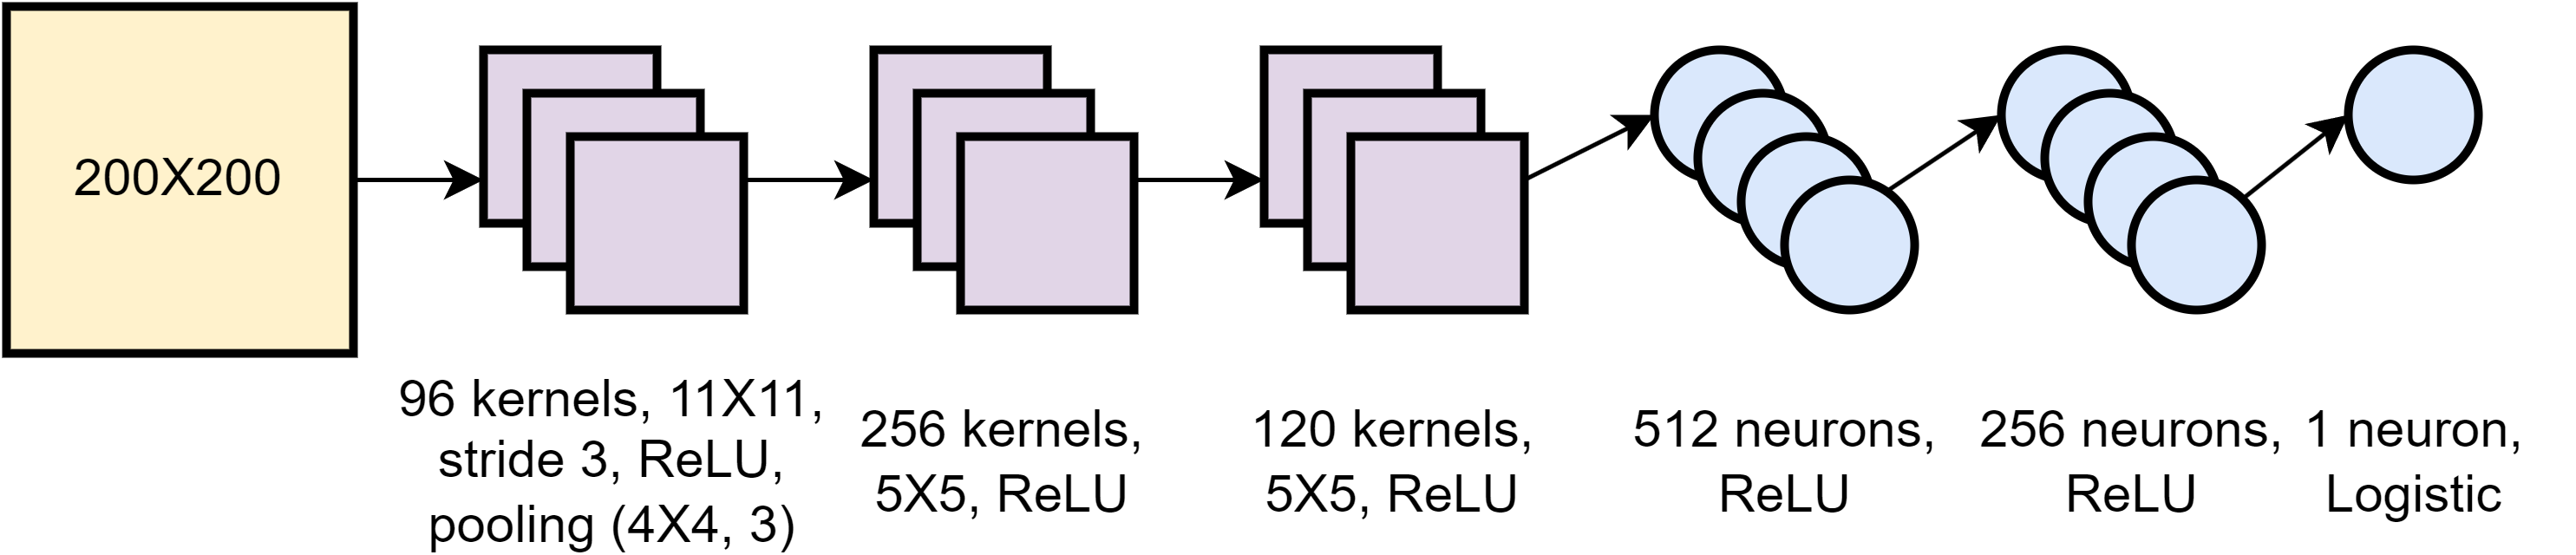
\includegraphics[width=17cm]{man-source/images/ch4/pic4-19.png}
	\caption{Сверточная нейронная сеть для определения наличия солнечных панелей}
	\label{fig:used_cnn}
\end{figure}

Для обучения были использованы изображения, полученные фотографированием со спутника (Google Maps). Для обучения и тестирования была использована выборка из 3347 3-канальных изображений размером 200Х200 пикселей (из которых 1643 содержали солнечные панели, а 1704 не содержали). Полная выборка делилась на обучающую и тестирующую выборки в соотношении 4 к 1. На рисунке \ref{fig:google_maps} отображены примеры используемых изображений.
 
\begin{figure}[ht]
	\centering
	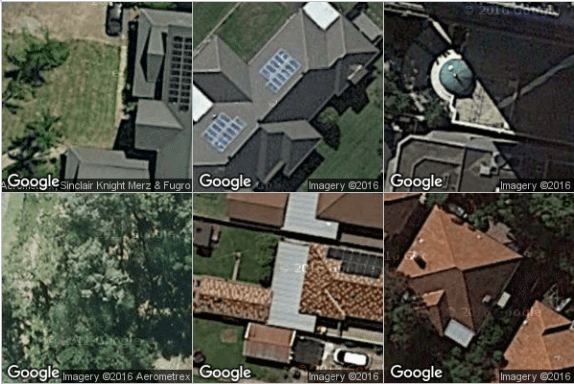
\includegraphics[width=12cm]{man-source/images/ch4/pic4-17.png}
	\caption{Примеры изображений, используемых для обучения}
	\label{fig:google_maps}
\end{figure}

Сеть обучалась на протяжении 70 эпох методом обратного распространения ошибки, при этом были использованы следующие параметры: скорость обучения -- 0,001, моментный параметр -- 0,9, weight-decay -- 0,0005, размер мини-батча -- 20, dropout с вероятностью 0,5 для полносвязных слоев сверточной нейронной сети.
	
В результате проведенных экспериментов была получена точность обнаружения объектов в 87.46\% (таблица \ref{table:solar_detection_cm} представляет confusion matrix, вычисленную для полученного бинарного классификатора на тестовой выборке).

\begin{table}[H]
	\caption{Confusion matrix для обученного классификатора}
	\label{table:solar_detection_cm}
	\centering
	\begin{tabular}{|p{6cm}|p{4cm}|p{4cm}|}
		\hline
		& \textbf{Предсказано отсутствие} & \textbf{Предсказано наличие}\\
		\hline
	    Фактически отсутствует & 325  & 32 \\
	    \hline
		Фактически присутствует & 52 & 261 \\
		\hline
	\end{tabular}			
\end{table}	

2. \textit{Для задачи распознавания маркировки} использовался конвейер нейронных сетей, каждая из которых решает определенную подзадачу:
\begin{easylistNum}
  & Оценка положения продукта в кадре;
	& Обнаружение продукта и маркировки;
	& Распознавание маркировки;
	& <<Сборка>> маркировки и ее проверка.
	Для достижения поставленных задач применялся конвейер, представленный на рисунке \ref{fig:general_diagram}.
\end{easylistNum}
 
\begin{figure}[!ht]
	\centering
	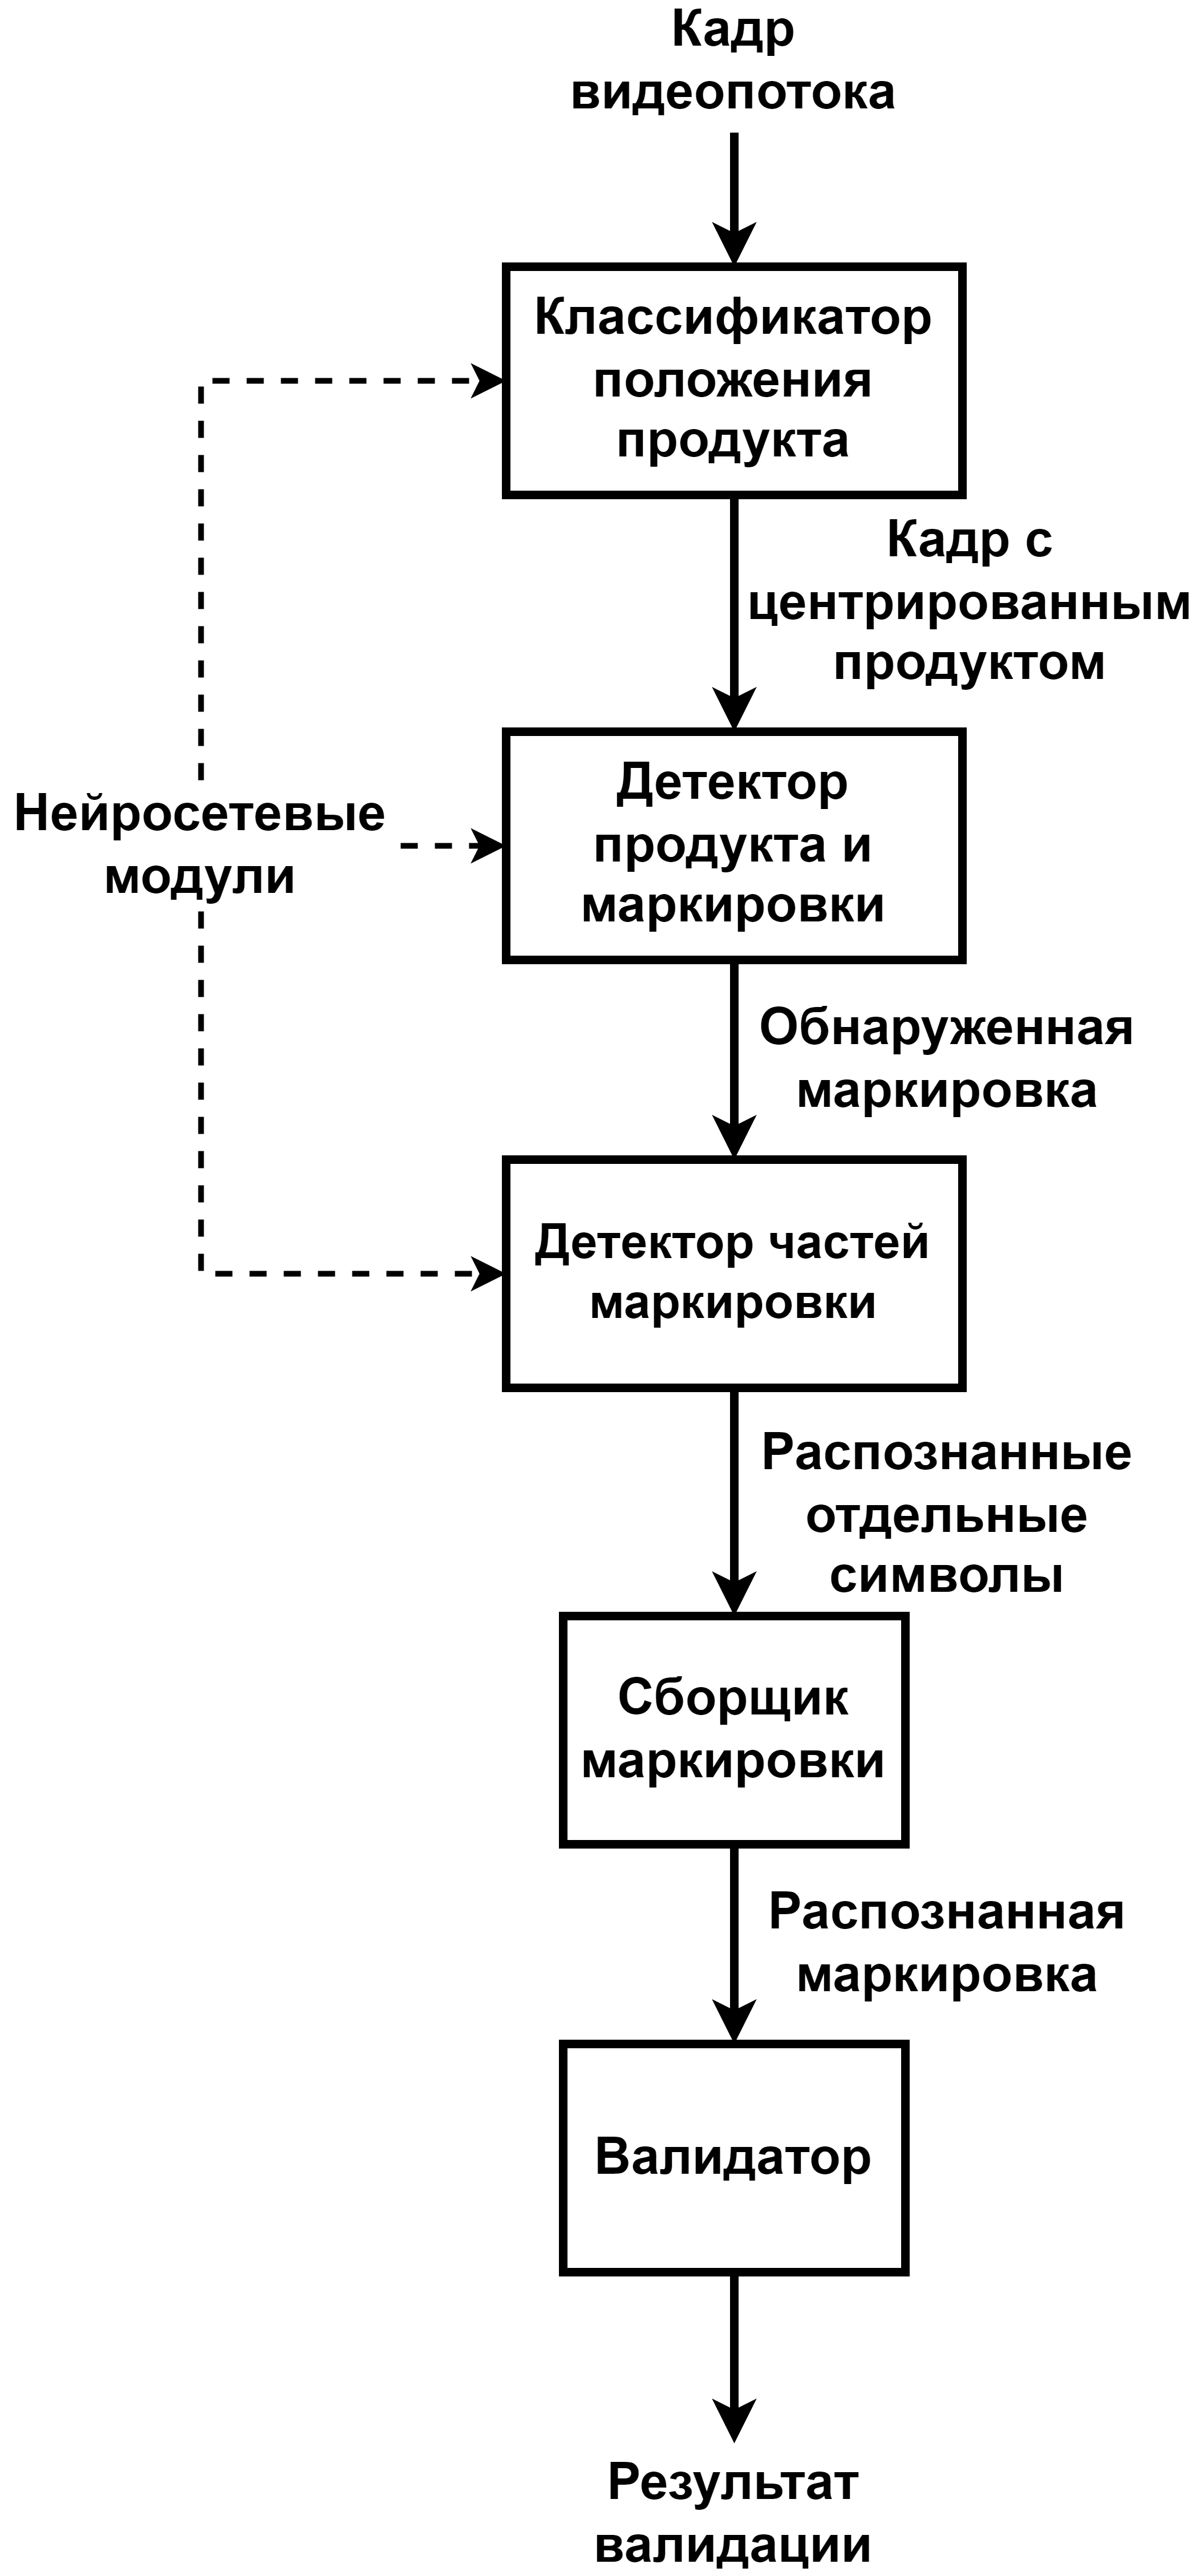
\includegraphics[width=8cm]{man-source/images/ch4/savushkin_structure.png}
	\caption{Конвейер нейросетевых моделей для распознавания маркировки}
	\label{fig:general_diagram}
\end{figure}

Применение предложенного конвейера нейросетевых моделей позволило осуществить независимую настройку и повысить эффективность работы отдельных моделей. Помимо этого, применяемые модели для оценки положения продукта в кадре позволили уменьшить количество обрабатываемых кадров видеопотока и, как следствие, увеличить скорость работы конвейера. Предложенный алгоритм может работать с разными типами маркировки (DataMatrix, QR, алфавитно-цифровая и т.д.).
	
В \textbf{\textit{заключении}} сформулированы основные научные результаты диссертации и рекомендации по их практическому применению.
Приложение содержит акты внедрения результатов диссертации и исходный код, реализующий метод предобучения глубокой нейронной сети.

\bigskip
\centerline{\bf ЗАКЛЮЧЕНИЕ}
\smallskip
{\bf Основные научные результаты диссертации}
\smallskip

\begin{enumerate}[wide, labelindent=10mm]

\item Выявлена и доказана эквивалентность задач максимизации функции правдоподобия распределения входных данных, минимизации суммарной квадратичной ошибки сети при использовании линейных нейронов и минимизации кросс-энтропийной функции ошибки сети в пространстве синаптических связей ограниченной машины Больцмана. Из полученных теоретических результатов следует, что природа неконтролируемого обучения в RBM-сети является идентичной при использовании различных целевых функций (\cite{2-A}, \cite{3-A}, \cite{4-A}, \cite{5-A}, \cite{10-A}, \cite{12-A}, \cite{13-A});
\item Разработан метод неконтролируемого предобучения глубоких нейронных сетей, базирующийся на минимизации квадратичной ошибки сети в скрытом и видимом слоях RBM-машины, что позволяет учитывать нелинейную природу нейронных элементов. Разработанный метод применен для обучения глубоких полносвязных и сверточных архитектур нейронных сетей и протестирован на выборках MNIST, CIFAR-10, CIFAR-100. Показано, что предложенный метод обладает большей эффективностью, чем классический (\cite{1-A}, \cite{2-A}, \cite{3-A}, \cite{4-A}, \cite{5-A}, \cite{10-A}, \cite{12-A}, \cite{13-A}, \cite{17-A}, \cite{18-A}, \cite{19-A}, \cite{20-A}, \cite{21-A}, \cite{22-A});
\item Предложен алгоритм редуцирования параметров глубокой нейронной сети, базирующийся на неконтролируемом предобучении сети и позволяющий сократить количество настраиваемых параметров сети и упростить ее архитектуру без потери обобщающей способности. Проведены вычислительные эксперименты, доказывающие эффективность предложенного метода (\cite{11-A}, \cite{16-A}, \cite{30-A});
\item С использованием предложенного метода предобучения реализованы прикладные нейросетевые системы компьютерного зрения. 

Разработана нейросетевая система обнаружения солнечных панелей на аэрофотоснимках, позволяющая обнаруживать солнечные панели с точностью 87,46\% с возможностью использования фотографий низкого разрешения (\cite{9-A}, \cite{14-A}, \cite{15-A}).

Разработана нейросетевая система распознавания маркировки продукта на производственной линии, базирующаяся на интеграции различных моделей глубоких сверточных нейронных сетей. Предложенный конвейер представляет собой цепочку взаимодействующих моделей нейросетевых классификаторов и детекторов, которые решают отдельные подзадачи обнаружения и распознавания маркировки или ее части. Подобная архитектура позволяет добавлять новые типы маркировок благодаря простой модульной структуре. Архитектуры нейросетей, используемые для построения конвейера, позволяют осуществлять обработку изображения в реальном времени (\cite{6-A}, \cite{7-A}, \cite{8-A}, \cite{23-A}, \cite{24-A}, \cite{25-A}, \cite{26-A}, \cite{27-A}, \cite{28-A}, \cite{29-A}).

% \item Разработан нейросетевой алгоритм детекции и распознавания лиц на фото и видеоизображениях, базирующийся на использовании предобученных сверточных нейронных сетей и позволяющий пополнять базу знаний интеллектуальной системы. Применение подобного подхода позволило добиться простой расширяемости системы распознавания лиц и высокой точности распознавания лиц, уже включенных в базу [\cite{28-A}, \cite{29-A}];

% \item Введено понятие гибридного решателя задач, обоснована актуальность согласованного использования нескольких моделей решения задач при решении комплексных задач. Сформулирована проблема совместимости различных моделей решения задач, препятствующая созданию гибридных решателей и технологий их разработки. Предложен ряд принципов, лежащих в основе комплекса моделей, методики и средств, который предлагается разрабатывать как часть технологии OSTIS. В качестве основы для построения гибридных решателей задач предлагается использовать вариант реализации многоагентного подхода, при котором агенты взаимодействуют между собой исключительно путем спецификации информационных процессов, выполняемых агентами в семантической памяти. \cite{7-A,3-A,12-A,13-A,14-A,18-A,19-A,26-A,34-A,36-A,37-A}.

% \item Предложена агентно-ориентированная модель гибридного решателя задач, рассматривающая каждый такой решатель как иерархическую систему агентов, управляемых ситуациями и событиями в общей семантической памяти,
% обеспечивающая модифицируемость таких решателей задач, а также возможность решения задач, требующих совместного использования различных методов решения задач. Предложенная модель позволяет рассматривать разрабатываемый решатель задач на различных уровнях детализации, что обеспечивает возможность поэтапного проектирования решателей, а также их модифицируемость. На основе предложенной модели гибридного решателя задач построена агентно-ориентированная модель интерпретатора базового языка программирования, ориентированного на обработку знаний \cite{4-A,5-A,1-A,3-A,14-A,15-A,16-A,18-A,20-A,21-A,26-A,28-A,31-A}.

% \item Предложена модель взаимодействия параллельных асинхронных информационных процессов в общей семантической памяти, определяющая принцип коммуникации агентов, выполняющих указанные процессы, включающая средства синхронизации процессов на основе механизма блокировок элементов семантической памяти, и обеспечивающая возможность спецификации планируемых блокировок, а также выявления и устранения взаимоблокировок. Уточнено понятие агента, выполняющего преобразования в семантической памяти. Разработана классификация агентов и средства их спецификации \cite{4-A,5-A,1-A,3-A,24-A,25-A,26-A,28-A,30-A,33-A}.

% \item Разработана методика построения и модификации гибридных решателей задач, построенных на основе предложенной модели решателя. В основе методики лежит формальная онтология действий разработчиков таких решателей. Наличие такой методики позволяет автоматизировать процесс построения и модификации решателей и снизить требования к их разработчикам. Указанная методика предполагает поэтапное проектирование гибридных решателей с учетом повторного использования разработанных ранее компонентов и возможности независимой отладки и верификации компонентов решателя на нескольких уровнях. \cite{6-A,8-A,2-A,11-A,14-A,15-A,17-A,23-A,26-A,32-A,35-A}.

% \item Разработаны средства автоматизации и информационной поддержки процесса построения и модификации гибридных решателей задач, включающие в себя систему автоматизации процесса построения и модификации решателей и подсистему информационной поддержки разработчиков решателей в рамках метасистемы IMS. Решатели задач каждой из подсистем построены на основе предложенной модели решателя, что обеспечивает их модифицируемость. Разработана библиотека многократно используемых компонентов решателей задач, включающая набор компонентов, языковые средства их спецификации и средства автоматизации поиска компонентов на основе заданной спецификации \cite{4-A,6-A,8-A,15-A,17-A,22-A,26-A}.

% \item С использованием языка C реализована разработанная агентно-ориентированная модель интерпретатора базового языка программирования, ориентированного на обработку знаний. Все описанные в рамках диссертационной работы модели формализованы и включены в состав соответствующих разделов базы знаний разрабатываемой метасистемы IMS, таким образом обеспечена информационная поддержка разработчиков решателей.
% С использованием предложенных моделей и средств разработаны решатели задач для ряда прикладных интеллектуальных систем. В процессе построения указанных решателей произведено стартовое наполнение библиотеки многократно используемых sc-агентов, показана эффективность предложенной методики с учетом текущей версии библиотеки. 
% Сведения об использовании результатов диссертационной работы отражены в соответствующих актах внедрения, приведенных в приложении к диссертации \cite{8-A,9-A,10-A,13-A,20-A,27-A,29-A,32-A,36-A}.

\end{enumerate}

\smallskip {\bf Рекомендации по практическому использованию результатов}\medskip


Результаты исследований использованы для практической реализации интеллектуальной системы видеонаблюдения реального времени. Научные и практические результаты диссертационной работы использованы в НИР, а также в ряде прикладных систем.

Предложенный метод предобучения глубоких нейронных сетей применялся при обучении нейросетевых компонентов для нейросетевой системы распознавания маркировки продукта на производственной линии ОАО <<Савушкин продукт>>.

Разработанные алгоритмы обнаружения и локализации солнечных панелей на аэрофотоснимках, методы предобучения нейросетевых моделей и инструментальные средства внедрены и используются в компании ООО <<Intelligent Semantic Systems>> при разработке интеллектуальной диалоговой системы в составе подсистемы компьютерного зрения.

Кроме того, научные и практические результаты диссертационной работы используются в учебном процессе учреждения образования <<Брестский государственный технический университет>>.

% Разработанные модели, средства и их программная реализация могут быть использованы при разработке решателей задач интеллектуальных систем различного назначения, как инструментальных, так и прикладных. 

Разработка проводилась с использованием свободного программного обеспечения и может быть использована в различных отечественных проектах без необходимости приобретения дорогостоящих программных средств.

% Научные и практические результаты диссертационной работы используются в учебном процессе учреждения образования <<Белорусский государственный университет информатики и радиоэлектроники>>, в НИЛ 3.7 при выполнении работ по договору БРФФИ--РФФИ (№ ГР 20164340), а также на предприятиях ОАО <<Савушкин продукт>> при разработке решателя задач системы автоматизации рецептурного производства, ООО <<ФордэКонсалтинг>> при разработке программной системы обслуживания клиентов розничной торговли, ООО <<Кинросс-ресерч>> при разработке системы автоматизации и оптимизации строительного проектирования, ФГБУН Институт систем энергетики им. Л. А. Мелентьева СО РАН при разработке решателя в области энергетики.

%\newpage

\def\selectlanguageifdefined#1{
\expandafter\ifx\csname date#1\endcsname\relax
\else\language\csname l@#1\endcsname\fi}

\bigskip
\centerline{\bf СПИСОК ПУБЛИКАЦИЙ СОИСКАТЕЛЯ УЧЕНОЙ СТЕПЕНИ}

\vspace{1mm}
{\bf Статьи в рецензируемых научных журналах}
\vspace{2mm}

\begin{enumerate}[wide, labelindent=10mm]

%\section*{Статьи в рецензируемых научных журналах}
\ifx\isabstract\undefined 
\section* {Статьи в научных рецензируемых изданиях, включенных в перечень изданий, и в иностранных научных изданиях}
\fi

\bibitem{1-A}
\selectlanguageifdefined{english}
Golovko, V. A Learning Technique for Deep Belief Neural Networks~/ V. Golovko, A. Kroshchanka, U. Rubanau, S. Jankowski~//
Neural Networks and Artificial Intelligence. ---
\newblock Cham: Springer International Publishing, 2014. ---
\newblock Vol.~440. Communication in Computer and Information Science. ---
\newblock P.~136--146.

\bibitem{2-A}
\selectlanguageifdefined{russian}
Головко, В. А. Персептроны и нейронные сети глубокого доверия: обучение и применение~/ В. А. Головко, А. А. Крощенко~//
  Вестник Брестского государственного технического университета. ---
\newblock Брест,~2014. ---
\newblock Т.~5. ---
\newblock {\cyr\CYRS.}~2--12.

\bibitem{3-A}
\selectlanguageifdefined{russian}
Головко, В. А. Метод обучения нейронной сети глубокого доверия и применение для визуализации данных~/ В. А. Головко, А. А. Крощенко~//
  Комп'ютерно-інтегровані технології: освіта, наука, виробництво. ---
\newblock Луцк,~2015. ---
\newblock Вып.~19. ---
\newblock {\cyr\CYRS.}~6--12.

\bibitem{4-A}
\selectlanguageifdefined{english}
Golovko, V. The nature of unsupervised learning in deep neural networks: A new understanding and novel approach~/ V. Golovko, A. Kroshchanka, D. Treadwell~//
  Optical Memory and Neural Networks. ---
\newblock New York : Allerton Press, Inc., 2016. ---
\newblock P.~127--141.

\bibitem{5-A}
\selectlanguageifdefined{russian}
Головко, В. А. Теория глубокого обучения: конвенциальный и новый подход~/ В. А. Головко, А. А. Крощенко, М. В. Хацкевич~//
  Вестник Брестского государственного технического университета. ---
\newblock Брест, 2016. ---
\newblock №~5. ---
\newblock {\cyr\CYRS.}~7--16.

\bibitem{6-A}
\selectlanguageifdefined{russian}
Головко, В. А. Интеграция искусственных нейронных сетей с базами знаний~/ В. А. Головко, В. В. Голенков, В. П. Ивашенко, В. В. Таберко, Д. С. Шаток, А. А. Крощенко, М. В. Ковалёв ~//
  Онтология проектирования. ---
\newblock EBSCO Publishing, 2018. ---
\newblock Т.~8. ---
\newblock №~3(29). ---
\newblock {\cyr\CYRS.}~366--386.

\bibitem{8-A}
\selectlanguageifdefined{english}
Golovko, V. Brands and caps labeling recognition in images using deep learning~/ V. Golovko, A. Kroshchanka, E. Mikhno~//
  International Conference on Pattern Recognition and Information Processing. ---
\newblock Cham: Springer International Publishing, 2019. ---
\newblock P.~35--51.

\bibitem{7-A}
\selectlanguageifdefined{russian}
Крощенко, А. А. Реализация нейросетевой системы распознавания маркировки продукции~/ А. А. Крощенко, В. А. Головко~//
  Вестник Брестского государственного технического университета. ---
\newblock Брест, 2019. ---
\newblock №~5. ---
\newblock {\cyr\CYRS.}~9--12.

\bibitem{28-A}
\selectlanguageifdefined{english}
Golovko, V. Neuro-Symbolic Artificial Intelligence: Application for Control the Quality of Product Labeling~/ V. Golovko, A. Kroshchanka, M. Kovalev, V. Taberko, D. Ivaniuk~// 
 International Conference on Open Semantic Technologies for Intelligent Systems. ---
\newblock Cham: Springer International Publishing, 2020. ---
\newblock P.~81--101.

\bibitem{10-A}
\selectlanguageifdefined{english}
Golovko,  V. A.  Deep Neural Networks: Selected Aspects of Learning and Application~/ V. A. Golovko, A. A. Kroshchanka, E. V. Mikhno~//
  Pattern Recognition and Image Analysis. ---
\newblock Berlin, Heidelberg : Springer-Verlag, 2021. ---
\newblock Vol.~31. ---
\newblock №~1. ---
\newblock P.~132--143.

\bibitem{9-A}
\selectlanguageifdefined{english}
Golovko, V. Deep convolutional neural network for detection of solar panels~/ V. Golovko, A. Kroshchanka, E. Mikhno, M. Komar, A. Sachenko~//
  Data-Centric Business and Applications. ---
\newblock Cham: Springer International Publishing, 2021. ---
\newblock P.~371--389.

\bibitem{29-A}
\selectlanguageifdefined{english}
Kroshchanka, A. Neural network component of the product marking recognition system on the production line~/ A. Kroshchanka, D. Ivaniuk~// 
 Open Semantic Technologies for Intelligent Systems (OSTIS-2021). ---
\newblock Minsk : BSUIR, 2021. ---
\newblock P.~219--224.

\bibitem{11-A}
\selectlanguageifdefined{english}
Kroshchanka, A. A. Method for Reducing Neural-Network Models of Computer Vision~/ A. A. Kroshchanka, V. A. Golovko, M. Chodyka~//
  Pattern Recognition and Image Analysis. ---
\newblock Berlin, Heidelberg : Springer-Verlag, 2022. ---
\newblock Vol.~32. ---
\newblock №~2. ---
\newblock P.~294--300.

\bibitem{30-A}
\selectlanguageifdefined{english}
Kroshchanka, A. Reduction of neural network models in intelligent computer systems of a new generation~/ A. Kroshchanka~// 
 Open Semantic Technologies for Intelligent Systems (OSTIS-2023). ---
\newblock Minsk : BSUIR, 2023. ---
\newblock P.~127--132.

\ifx\isabstract\undefined 
\begin{center}
\vspace{3mm}
{\bf Статьи в других научных изданиях}
\vspace{3mm}
\end{center}
\else
\vspace{2mm}
{\bf Статьи в других научных изданиях}
\vspace{2mm}
\fi

\bibitem{23-A}
\selectlanguageifdefined{english}
Golovko, V. A. Integration of artificial neural networks and knowledge bases~/ V. A. Golovko, A. A. Kroshchanka, V. V. Golenkov, V. P. Ivashenko, M. V. Kovalev, V. V. Taberko, D. S. Ivaniuk~// 
 Open Semantic Technologies for Intelligent Systems (OSTIS-2018). ---
\newblock Minsk : BSUIR, 2018. ---
\newblock P.~133--146.

\bibitem{25-A}
\selectlanguageifdefined{english}
Golovko, V. Principles of decision-making systems building based on the integration of neural networks and semantic models~/ V. Golovko, A. Kroshchanka, V. Ivashenko, M. Kovalev, V. Taberko, D. Ivaniuk~//
 Open Semantic Technologies for Intelligent Systems (OSTIS-2019). ---
\newblock Minsk : BSUIR, 2019. ---
\newblock P.~91--102.

\bibitem{27-A}
\selectlanguageifdefined{english}
Golovko, V. Implementation of an intelligent decision support system to accompany the manufacturing process~/ V. Golovko, A. Kroshchanka, M. Kovalev, V. Taberko, D. Ivaniuk~// 
 Open Semantic Technologies for Intelligent Systems (OSTIS-2020). ---
\newblock Minsk : BSUIR, 2020. ---
\newblock P.~175--182.

%\section*{Статьи в сборниках материалов научных конференций}
\ifx\isabstract\undefined 
\begin{center}
\vspace{3mm}
{\bf Статьи в сборниках материалов научных конференций}
\vspace{3mm}
\end{center}
\else
\vspace{2mm}
{\bf Статьи в сборниках материалов научных конференций}
\vspace{2mm}
\fi

\bibitem{12-A}
\selectlanguageifdefined{english}
Golovko, V. A New Technique for Restricted Boltzmann Machine Learning~/ A. Kroshchanka, V. Turchenko, S. Jankowski, D. Treadwell~//
  Proceedings of the 8th IEEE International Conference IDAACS-2015, Warsaw 24-26 September 2015. ---
\newblock Warsaw, 2015. ---
\newblock P.~182--186.

\bibitem{19-A}
\selectlanguageifdefined{russian}
Головко, В. А. Применение нейронных сетей глубокого доверия для выделения семантически значимых признаков~/ В. А. Головко, А. А. Крощенко~// 
 Открытые семантические технологии проектирования интеллектуальных систем (OSTIS-2015) : материалы V междунар. науч.-техн. кофн. ---
\newblock Минск : БГУИР, 2015. ---
\newblock P.~481--486.

\bibitem{20-A}
\selectlanguageifdefined{russian}
Крощенко, А. А. Применение нейронных сетей глубокого доверия в интеллектуальном анализе данных~/ А. А. Крощенко~// 
 сборник материалов IX Республиканской научной конференции молодых ученых и студентов <<Современные проблемы математики и вычислительной техники>>. ---
\newblock Брест : БрГТУ, 2015. ---
\newblock {\cyr\CYRS.}~12--14.

\bibitem{13-A}
\selectlanguageifdefined{english}
Golovko, V. Theoretical Notes on Unsupervised Learning in Deep Neural Networks~/ V. Golovko, A. Kroshchanka~//
  Proceedings of the 8th International Joint Conference on Computational Intelligence (IJCCI 2016). ---
\newblock SCITEPRESS, 2016. ---
\newblock P.~91--96.

\bibitem{14-A}
\selectlanguageifdefined{russian}
Golovko, V. Convolutional neural network based solar photovoltaic panel detection in satellite photos~/ V. Golovko, S. Bezobrazov, A. Kroshchanka, A. Sachenko, M. Komar, A. Karachka~//
  9th IEEE International Conference on Intelligent Data Acquisition and Advanced Computing Systems: Technology and Applications (IDAACS). ---
\newblock IEEE, 2017. ---
\newblock Vol.~1. ---
\newblock P.~14--19.

\bibitem{15-A}
\selectlanguageifdefined{russian}
Golovko, V. Development of solar panels detector~/ V. Golovko, A. Kroshchanka, S. Bezobrazov, A. Sachenko, M. Komar, O. Novosad~//
  International Scientific-Practical Conference Problems of Infocommunications. Science and Technology (PIC S\&T). ---
\newblock IEEE, 2018. ---
\newblock P.~761--764.

\bibitem{24-A}
\selectlanguageifdefined{russian}
Головко, В. А. Нейросетевые модели глубокого обучения для решения задач распознавания объектов на изображении~/ В. А. Головко, А. А. Крощенко~//
 Вычислительные методы, модели и образовательные технологии : сборник материалов VII международной научно-практической конференции. ---
\newblock Брест : БрГУ, 2018. ---
\newblock {\cyr\CYRS.}~3--5. 

\bibitem{26-A}
\selectlanguageifdefined{russian}
Головко, В. А. Обнаружение и распознавание маркировки продукции с помощью нейросетевых алгоритмов~/ В. А. Головко, А. А. Крощенко~//
 Вычислительные методы, модели и образовательные технологии : сборник материалов VIII международной научно-практической конференции. ---
\newblock Брест : БрГУ, 2019. ---
\newblock {\cyr\CYRS.}~3--6. 

\bibitem{16-A}
\selectlanguageifdefined{russian}
Kroshchanka, A. The Reduction of Fully Connected Neural Network Parameters Using the Pre-training Technique~/ A. Kroshchanka, V. Golovko~//
  11th IEEE International Conference on Intelligent Data Acquisition and Advanced Computing Systems: Technology and Applications (IDAACS). ---
\newblock IEEE, 2021. ---
\newblock Vol.~2. ---
\newblock P.~937--941.

% \bibitem{28-A}
% \selectlanguageifdefined{english}
% Kroshchanka, A. Semantic analysis of the video stream based on neuro-symbolic artificial intelligence~/ A. Kroshchanka, E. Mikhno, M. Kovalev, V. Zahariev, A. Zagorskij~// 
%  Open Semantic Technologies for Intelligent Systems (OSTIS-2021). ---
% \newblock Minsk : BSUIR, 2021. ---
% \newblock №~5. ---
% \newblock P.~193--204.

% \bibitem{29-A}
% \selectlanguageifdefined{russian}
% Головко, В. А. Гибридная интеллектуальная система оценки эмоционального состояния пользователя~/ В. А. Головко, А. А. Крощенко~// 
%  Современные проблемы математики и вычислительной техники : сборник материалов ХII Республиканской научной конференции молодых ученых и студентов, Брест, 18–19 ноября 2021 г.~/ Министерство образования Республики Беларусь, Брестский государственный технический университет ; редкол.: В. А. Головко (гл. ред.) [и др.]. ---
% \newblock Брест : БрГТУ, 2021. ---
% \newblock {\cyr\CYRS.}~10--13.

% \bibitem{24-A}
% \selectlanguageifdefined{russian}
% Формальное семантическое описание целенаправленной деятельности различного вида субъектов~/ Д. В. Шункевич,  А. В. Губаревич, М.~Н.~Святкина, О. Л. Моросин~// 
%  Открытые семантические технологии проектирования интеллектуальных систем (OSTIS-2016) : материалы VI Междунар. науч.-техн. конф., Минск, 18–20 февр. 2016 г.~/ Белорус. гос. ун-т информатики и радиоэлектроники ; редкол.: В. В. Голенков (отв. ред.) [и др.]. ---
% \newblock Минск, 2016. ---
% \newblock {\cyr\CYRS.}~125--136.

% \bibitem{25-A}
% \selectlanguageifdefined{russian}
% Шункевич, Д. В. Взаимодействие асинхронных параллельных процессов обработки знаний в общей семантической памяти~/ Д. В. Шункевич~// 
%  Открытые семантические технологии проектирования интеллектуальных систем (OSTIS-2016) : материалы VI Междунар. науч.-техн. конф., Минск, 18–20 февр. 2016 г.~/ Белорус. гос. ун-т информатики и радиоэлектроники ; редкол.: В. В. Голенков (отв. ред.) [и др.]. ---
% \newblock Минск, 2016. ---
% \newblock {\cyr\CYRS.}~137--144.

% \bibitem{26-A}
% \selectlanguageifdefined{english}
% Shunkevich, D. Ontology-based design of knowledge processing machines~/ D. Shunkevich~// 
%   Открытые семантические технологии проектирования интеллектуальных систем : материалы междунар. науч.-техн. конф., Минск, 16–18 февр. 2017 г.~/ Белорус. гос. ун-т информатики и радиоэлектроники ; редкол.: В. В. Голенков (отв. ред.) [и др.]. ---
% \newblock Минск, 2017. --- Вып. 1. ---
% \newblock P.~73--94.

% \bibitem{27-A}
% \selectlanguageifdefined{english}
% Ontology-based design of batch manufacturing enterprises~/ V.~Golenkov, K.~Rusetski, D.~Shunkevich, I.~Davydenko, V.~Zakharov, V.~Ivashenko, D.~Koronchik, V.~Taberko, D.~Ivanyuk~// 
%   Открытые семантические технологии проектирования интеллектуальных систем : материалы междунар. науч.-техн. конф., Минск, 16–18 февр. 2017 г.~/ Белорус. гос. ун-т информатики и радиоэлектроники ; редкол.: В. В. Голенков (отв. ред.) [и др.]. ---
% \newblock Минск, 2017. --- Вып.~1. ---
% \newblock С.~265--280.

% \bibitem{28-A}
% \selectlanguageifdefined{russian}
% Семантическая модель представления и обработки баз знаний~/ В.~В.~Голенков, Н. А. Гулякина, И. Т. Давыденко, Д. В. Шункевич~// 
%  Аналитика и управление данными в областях с интенсивным использованием данных : сб. науч. тр. XIX Междунар. конф. DAMDID/RCDL’2017, Москва, 10–13 окт. 2017 г. / Федер. исслед. центр <<Информатика и управление>> Рос. акад. наук ; под ред. Л. А. Калиниченко [и др.]. ---
% \newblock М., 2017. ---
% \newblock {\cyr\CYRS.}~412--419.

%\section*{Статьи в сборниках материалов научных конференций}
\ifx\isabstract\undefined 
\begin{center}
\vspace{3mm}
{\bf Тезисы}
\vspace{3mm}
\end{center}
\else
\vspace{2mm}
%\newpage
{\bf Тезисы}
\vspace{2mm}
\fi

\bibitem{17-A}
\selectlanguageifdefined{russian}
Крощенко, А. А. Методы глубокого обучения нейронных сетей~/ А.А. Крощенко~// 
 Материалы конференции <<Вычислительные методы, модели и образовательные технологии>>. ---
\newblock Брест : БрГУ, 2013. ---
\newblock {\cyr\CYRS.}~21--22.

\bibitem{18-A}
\selectlanguageifdefined{russian}
Головко, В. А. Об одном методе обучения нейронных сетей глубокого доверия~/ В. А. Головко, А. А. Крощенко~// 
 Вычислительные методы, модели и образовательные технологии : сборник материалов международной научно-практической конференции. ---
\newblock Брест : БрГУ, 2014. ---
\newblock {\cyr\CYRS.}~98--99.

\bibitem{21-A}
\selectlanguageifdefined{russian}
Головко, В. А.  Применение нейронных сетей глубокого доверия в интеллектуальном анализе данных~/ В. А. Головко, А. А. Крощенко~// 
 Вычислительные методы, модели и образовательные технологии : сборник материалов международной научно-практической конференции. ---
\newblock Брест : БрГУ, 2015.---
\newblock {\cyr\CYRS.}~97--98.

\bibitem{22-A}
\selectlanguageifdefined{russian}
Крощенко, А. А. Применение глубокой нейронной сети для решения задачи распознавания образов~/ А. А. Крощенко~// 
 Вычислительные методы, модели и образовательные технологии : сборник материалов международной научно-практической конференции. ---
\newblock Брест : БрГУ, 2016.---
\newblock {\cyr\CYRS.}~132--133.

% \bibitem{29-A}
% \selectlanguageifdefined{russian}
% Интеллектуальный решатель задач по геометрии~/ Д. В. Шункевич, С. С.~Заливако, О. Ю.~Савельева, С. С.~Старцев~// 
%   Информационные системы и технологии IST’2010 : материалы VI Междунар. конф., Минск, 24–25 нояб. 2010 г. / Белорус. гос. ун-т [и др.] ; редкол.: А. Н. Курбацкий (отв. ред.) [и др.]. ---
% \newblock Минск, 2010. ---
% \newblock {\cyr\CYRS.}~482--485.

% \bibitem{30-A}
% \selectlanguageifdefined{russian}
% Шункевич, Д. В.  Принципы проектирования и интерпретации программ, ориентированных на обработку семантических сетей~/ Д. В. Шункевич~// 
%  Информационные технологии и системы-2013 (ИТС 2013) : материалы междунар. науч. конф., Минск, 23 окт. 2013 г.~/ Белорус. гос. ун-т информатики и радиоэлектроники ; редкол.: \mbox{Л. Ю.} Шилин (гл. ред) [и др.]. ---
% \newblock Минск, 2013. ---
% \newblock {\cyr\CYRS.}~116--117.

% \bibitem{31-A}
% \selectlanguageifdefined{russian}
% Шункевич, Д. В.  Базовые понятия технологии компонентного проектирования машин обработки знаний систем дистанционного обучения~/ \mbox{Д. В. Шункевич}~// 
%   Дистанционное обучение -- образовательная среда XXI века : материалы VIII междунар. науч.-метод. конф., Минск, 5–6 дек. 2013г. / Белорус. гос. ун-т информатики и радиоэлектроники ; редкол.: Б. В. Никульшин [и др.]. ---
% \newblock Минск, 2013. ---
% \newblock {\cyr\CYRS.}~186--187.

% \bibitem{32-A}
% \selectlanguageifdefined{russian}
% Якимчик, С. В.  Принципы построения решателей задач в прикладных интеллектуальных системах~/ С. В. Якимчик, Д. В. Шункевич~// 
%  Информационные технологии и системы-2014 (ИТС 2014) : материалы междунар. науч. конф., Минск, 29 окт. 2014 г.~/ Белорус. гос. ун-т информатики и радиоэлектроники ; редкол.: \mbox{Л. Ю.} Шилин (гл. ред.) [и др.]. ---
% \newblock Минск, 2014. ---
% \newblock {\cyr\CYRS.}~160--161.

% \bibitem{33-A}
% \selectlanguageifdefined{russian}
% Губаревич, А. В.  Онтология деятельности интеллектуальных агентов над общей памятью~/ А. В. Губаревич, М. Н. Святкина Д. В. Шункевич~// 
%  Информационные технологии и системы-2015 (ИТС 2015) : материалы междунар. науч. конф., Минск, 28 окт. 2015 г.~/ Белорус. гос. ун-т информатики и радиоэлектроники ; редкол.: \mbox{Л. Ю.} Шилин (гл. ред.) [и др.]. ---
% \newblock Минск, 2015. ---
% \newblock {\cyr\CYRS.}~138--139.

% \bibitem{34-A}
% \selectlanguageifdefined{russian}
% Онтологическое моделирование для реализации семантических технологий создания интеллектуальной системы управления жизненным циклом~/ А. В. Федотова, И. Т. Давыденко, М. Н. Святкина, Д. В. Шункевич~// 
%     Информационная безопасность регионов России (ИБРР–2015) : IX С.-Петерб. межрегион. конф., Санкт-Петербург, 28–30 окт. 2015 г. : материалы конф. / \mbox{С.-Петерб.} О-во информатики, вычисл. техники, систем связи и упр ; редкол.: Б. Я. Советов [и др.].  ---
% \newblock СПб., 2015. ---
% \newblock {\cyr\CYRS.}~336.

% \bibitem{35-A}
% \selectlanguageifdefined{russian}
% Шункевич, Д. В.  Унифицированная семантическая модель процесса проектирования машин обработки знаний~/ Д. В. Шункевич, И. Б. Фоминых, О. Л. Моросин~// 
%  Информационные технологии и системы-2016 (ИТС 2016) : материалы междунар. науч. конф., Минск, 26 окт. 2016 г.~/ Белорус. гос. ун-т информатики и радиоэлектроники ; редкол.: \mbox{Л. Ю.} Шилин (гл. ред.) [и др.]. ---
% \newblock Минск, 2016. ---
% \newblock {\cyr\CYRS.}~172--173.

% \bibitem{36-A}
% \selectlanguageifdefined{russian}
% Шункевич, Д. В.  Представление базовых конструкций языка семантических сетей с теоретико-множественной интерпретацией средствами платформы Neo4j~/ Д. В. Шункевич, О. С. Родионова~// 
%  Информационные технологии и системы-2016 (ИТС 2016) : материалы междунар. науч. конф., Минск, 26 окт. 2016 г.~/ Белорус. гос. ун-т информатики и радиоэлектроники ; редкол.: \mbox{Л. Ю.} Шилин (гл. ред.) [и др.]. ---
% \newblock Минск, 2016. ---
% \newblock {\cyr\CYRS.}~174--175.

% \bibitem{37-A}
% \selectlanguageifdefined{russian}
% Голенков, В. В. Принципы построения машин обработки баз знаний~/ В. В. Голенков, Д. В. Шункевич~// 
%  Информационные технологии и системы-2017 (ИТС 2017) : материалы междунар. науч. конф., Минск, 25 окт. 2017 г.~/ Белорус. гос. ун-т информатики и радиоэлектроники ; редкол.: \mbox{Л. Ю.} Шилин (гл. ред.) [и др.]. ---
% \newblock Минск, 2017. ---
% \newblock {\cyr\CYRS.}~134--135.

\end{enumerate}

\newpage
\begin{center}
\bf РЕЗЮМЕ
\\[1mm]\rm Крощенко Александр Александрович\\[1mm] \bf
МЕТОДЫ ОБУЧЕНИЯ ГЛУБОКИХ НЕЙРОННЫХ СЕТЕЙ ДЛЯ ЗАДАЧ КОМПЬЮТЕРНОГО ЗРЕНИЯ
 \end{center}

{\bf Ключевые слова}: глубокие нейронные сети, компьютерное зрение, сверточные нейронные сети, ограниченная машина Больцмана, детекция объектов

\textbf{Целью работы} является разработка методов и алгоритмов для обучения глубоких нейронных сетей, применяемых для решения прикладных задач компьютерного зрения.

\textbf{Принципы и методы исследования}: в работе использовались методы теории нейронных сетей и машинного обучения, методы обработки изображений, детекции и распознавания образов.

\textbf{Полученные результаты и их новизна}.
Разработан метод неконтролируемого предобучения глубоких нейронных сетей, позволяющий учитывать нелинейную природу нейронных элементов. Разработан алгоритм, позволяющий сократить количество настраиваемых параметров сети. Для демонстрации эффективности предложенных метода и алгоритма проведены вычислительные эксперименты с использованием выборок компьютерного зрения MNIST, CIFAR-10 и CIFAR-100.

Доказана теорема, что максимизация функции правдоподобия распределения входных данных в пространстве синаптических связей ограниченной машины Больцмана эквивалентна минимизации кросс-энтропии функции ошибки сети и минимизации суммарной квадратичной ошибки сети при использовании линейных нейронов.

Полученные теоретические результаты использовались при разработке практических решений в области компьютерного зрения.

Предложена нейросетевая система обнаружения солнечных панелей на аэрофотоснимках, базирующаяся на использовании сверточных нейронных сетей.

Для распознавания маркировки продукта на производственной линии предложена нейросетевая система, основывающаяся на применении конвейера нейросетевых моделей для решения отдельных подзадач обработки, который позволил осуществлять анализ маркировки в реальном времени.

\textbf{Рекомендации к использованию и область применения}:
интеллектуальные системы видеонаблюдения, используемые для анализа маркировки продукта на производственных линиях и анализа аэрофотоснимков.

\newpage
\begin{center}
\bf РЭЗЮМЭ\\[1mm]\rm Крашчанка Аляксандр Аляксандравіч\\[1mm] \bf МЕТАДЫ НАВУЧАННЯ ГЛЫБОКIХ НЕЙРОНАВЫХ СЕТАК ДЛЯ ЗАДАЧ КАМП'ЮТЭРНАГА ЗРОКУ
\end{center}

{\bf Ключавыя словы}: глыбокія нейронавыя сеткі, камп'ютэрны зрок, згортачныя нейронавыя сеткі, гібрыдныя інтэлектуальныя сістэмы, абмежаваная машына Больцмана, дэтэкцыя аб'екта\u{у}.

\textbf{Мэта працы}: распрацо\u{у}ка метада\u{у} і алгарытма\u{у} для навучання глыбокіх нейронавых сетак, якія выкарысто\u{у}ваюцца для вырашэння прыкладных задач камп'ютэрнага зроку.

\textbf{Прынцыпы i метады даследавання}: у працы выкарысто\u{у}валіся метады тэорыі нейронавых сетак і машыннага навучання, метады апрацо\u{у}кі відарыса\u{у}, дэтэкцыі і распазнанні выя\u{у}.

\textbf{Атрыманыя вынiкi i iх навiзна}.
Распрацаваны метад некантралюемага праднавучання глыбокіх нейронавых сетак, які дазваляе улічваць нелінейную прыроду нейронавых элемента\u{у}. Распрацаваны алгарытм, які дазваляе скараціць колькасць наладжвальных параметра\u{у} сеткі. Для дэманстрацыі эфекты\u{у}насці прапанаваных метаду і алгарытму праведзены вылічальныя эксперыменты з выкарыстаннем агульнавядомых выбарак камп'ютарнага зроку MNIST, CIFAR-10 і CIFAR-100.

Даказаная тэарэма, што максімізацыя функцыі пра\u{у}дападабенства размеркавання \u{у}ваходных дадзеных у прасторы сінаптычных сувязя\u{у} абмежаванай машыны Больцмана эквівалентная мінімізацыі крос-энтрапіі функцыі памылкі сеткі і мінімізацыі сумарнай квадратычнай памылкі сеткі пры выкарыстанні лінейных нейрона\u{у}.

Атрыманыя тэарэтычныя вынікі выкарысто\u{у}валіся пры распрацо\u{у}цы практычных рашэння\u{у} у вобласці кампутарнага зроку.

Прапанавана нейросеткавая сістэма выяўлення сонечных панэля\u{у} на аэрафотаздымках, які базуецца на выкарыстанні згортачнай нейронавай сеткі.

Для распазнання маркіро\u{у}кі прадукта на вытворчай лініі прапанавана нейросеткавая сістэма, якая засно\u{у}ваецца на \u{у}жыванні канвеера нейрасеткавых мадэля\u{у} для рашэння асобных падзадач апрацо\u{у}кі, які дазваляе ажыцця\u{у}ляць аналіз маркіро\u{у}кі \u{у} рэальным часе.
	
\textbf{Рэкамендацыi па выкарыстаннi i вобласць ужывання}:
інтэлектуальныя сістэмы відэаназірання, якія выкарысто\u{у}ваюцца для аналізу маркіро\u{у}кі прадукта на вытворчых лініях i аналіза аэрафотаздымка\u{у}.

\newpage
\begin{center}
\bf SUMMARY\\[1mm]\rm Kroshchenko Aleksandr Aleksandrovich\\[1mm] \bf
METHODS FOR TRAINING DEEP NEURAL NETWORKS FOR COMPUTER VISION PROBLEMS
\end{center}

{\bf Keywords:} deep neural networks, computer vision, convolutional neural networks, hybrid intelligent systems, restricted Boltzmann machine, object detection.

\textbf{The purpose of the work } is development of methods and algorithms for training deep neural networks used to solve applied problems of computer vision.

\textbf{Principles and methods of research}: the methods of the theory of neural networks and machine learning, methods of image processing, detection and pattern recognition were used in the work.

\textbf{The obtained results and their novelty}.
A method for unsupervised pretraining of deep neural networks has been developed, which allows taking into account the nonlinear nature of neural elements. An algorithm has been developed to reduce the number of tunable neural network parameters. To demonstrate the effectiveness of the proposed method and algorithm, computational experiments were carried out using computer vision datasets MNIST, CIFAR-10 and CIFAR-100.

The theorem is proven that maximizing the likelihood function of the distribution of input data in the space of synaptic connections of a limited Boltzmann machine is equivalent to minimizing the cross-entropy of the network error function and minimizing the total squared error of the network when using linear neurons.

The theoretical results obtained were used to develop practical solutions in the area of computer vision.

A neural network system for detecting solar panels on aerial photographs is proposed, based on the use of convolutional neural networks.

To recognize product markings on a production line, a neural network system is proposed, based on the use of a pipeline of neural network models to solve separate processing subtasks, which made it possible to analyze markings in real time.

% Methods for unsupervised pre-training of deep neural networks have been developed, which make it possible to take into account the nonlinear nature of neural elements and reduce the number of adjustable network parameters. To demonstrate the effectiveness of the proposed methods, computational experiments were carried out using well-known computer vision datasets MNIST and CIFAR-10.
	
% A theorem is proved that maximizing the likelihood function of the distribution of input data in the space of synaptic connections of a restricted Boltzmann machine is equivalent to minimizing the cross-entropy of the network error function and minimizing the total quadratic error of the network when using linear neurons.
	
% The obtained theoretical results were used in the development of practical solutions in the field of computer vision.
	
% To determine the presence of solar panels in aerial photographs, an algorithm based on the use of a convolutional neural network is proposed.
	
% To recognize product labeling on a production line, an algorithm is proposed based on the use of a pipeline of neural network models to solve individual processing subtasks, which allows real-time analysis of markings.
	
% A neural network algorithm for detecting and recognizing faces in photo and video images has been developed, based on the use of pre-trained convolutional neural networks and allowing to renew the knowledge base of an intelligent system.

\textbf{Recommendations on the use and field of application:}
intelligent video surveillance systems used to analyze product labeling on production lines, analysis of aerial photographs, intelligent face identification systems with the possibility of automatic additional training.

\newpage
\thispagestyle{empty}

\vspace* {0.5cm}

\begin{center}
\textit{Научное издание}

\vspace*{\fill}

\textbf{Крощенко} Александр Александрович\\[25mm]
 {\large\bf МЕТОДЫ ОБУЧЕНИЯ ГЛУБОКИХ НЕЙРОННЫХ СЕТЕЙ ДЛЯ ЗАДАЧ КОМПЬЮТЕРНОГО ЗРЕНИЯ \\}
 
\vspace* {2cm}

 
АВТОРЕФЕРАТ
 
диссертации на соискание ученой степени кандидата технических наук

\vspace* {1cm}

по специальности 05.13.17 — Теоретические основы информатики

\end{center}

\vspace*{\fill}\vspace*{\fill} \vspace*{\fill} \vspace*{\fill}
\begin{tabbing}
XXXXXXXXXXXXXXXXXXXXXXXXXXXXXX\= \kill
\end{tabbing}

\begin{center}

%{\small \mbox{%Подписано в печать %~~~~.06.2018 г. Формат $60\times84\ \  1/16$. Бумага офсетная. Гарнитура «Таймс».}\\
%Отпечатано на ризографе. Усл. печ. 1,63. Уч.-изд. л. 1,5. Тираж 60 экз. Заказ ~~~~.

%\bigskip
%Учетн. изд. л. 1.2. Тираж 60 экз. ~ Заказ № \hspace{8mm}.\\

%Издатель и полиграфическое исполнение: %учреждение образования \\
%«Белорусский государственный университет информатики и радиоэлектроники». \\
%Свидетельство о государственной регистрации издателя, изготовителя, распространителя печатных изданий № %1/238 от 24.03.2014,\\ 
%№ 2/113 от 07.04.2014, № 3/615 от 07.04.2014. \\
%ЛП № 02330/264 от 14.04.2014.\\
%220013, Минск, П. Бровки, 6
%}
\end{center}
\end{document}
